% ============================================================
% IEEE TEMSMET 2026 — FINAL PRODUCTION MANUSCRIPT
% Document class: IEEEtran (conference, two-column, A4)
% Compiled with: pdflatex → bibtex → pdflatex → pdflatex
% IEEEtran.cls is included in TeX Live / MiKTeX by default.
% Figure path: ../../outputs/figures/ (relative to docs/paper/)
% Reference numbering: IEEE appearance order (renumbered from
%   thematic order in final_submission_manuscript.md)
% ============================================================

\documentclass[conference,a4paper]{IEEEtran}

% --- Core packages ----------------------------------------
\usepackage[T1]{fontenc}
\usepackage[utf8]{inputenc}
\usepackage{amsmath,amssymb}
\usepackage{graphicx}
\usepackage{booktabs}
\usepackage{array}
\usepackage{multirow}
\usepackage{url}
\usepackage{xspace}
\usepackage{cite}
\usepackage[hidelinks]{hyperref}

% --- Figure path ------------------------------------------
\graphicspath{{../../outputs/figures/}}

% --- Convenience macros -----------------------------------
\newcommand{\SHAP}{\textsc{shap}\xspace}
\newcommand{\LIME}{\textsc{lime}\xspace}
\newcommand{\NIDS}{NIDS\xspace}
\newcommand{\SMOTE}{SMOTE\xspace}
\newcommand{\XAI}{XAI\xspace}
\newcommand{\rbs}{rank-biserial~$r$\xspace}
\newcommand{\cohensh}{Cohen's~$h$\xspace}

% ==========================================================
\begin{document}
% ==========================================================

\title{Impact of SMOTE-Based Class Rebalancing on SHAP\\ and LIME
       Explanation Quality in Random Forest\\ Network Intrusion Detection}

% --- Author block (REPLACE PLACEHOLDERS BEFORE SUBMISSION) -
\author{%
  \IEEEauthorblockN{Author One\IEEEauthorrefmark{1},
                    Author Two\IEEEauthorrefmark{2},
                    Author Three\IEEEauthorrefmark{1}}
  \IEEEauthorblockA{\IEEEauthorrefmark{1}%
    Department of [DEPARTMENT], [INSTITUTION], [City], [Country]\\
    Email: \{author1, author3\}@[domain]}
  \and
  \IEEEauthorblockA{\IEEEauthorrefmark{2}%
    Department of [DEPARTMENT], [INSTITUTION], [City], [Country]\\
    Email: author2@[domain]}
}

\maketitle

% ----------------------------------------------------------
\begin{abstract}
Machine learning--based Network Intrusion Detection Systems (\NIDS) routinely
apply the Synthetic Minority Over-sampling Technique (\SMOTE) to address severe
traffic-class imbalance, yet the impact of such rebalancing on post-hoc
explainability outputs has not been systematically quantified in the \NIDS
literature. This study investigates how \SMOTE rebalancing affects the feature
attribution rankings produced by SHapley Additive exPlanations (SHAP) and Local
Interpretable Model-agnostic Explanations (LIME) in a Random Forest \NIDS trained
and evaluated on the UNSW-NB15 benchmark dataset. Two Random Forest classifiers
--- one trained on the original imbalanced partition and one on a \SMOTE-rebalanced
partition --- are evaluated against the same 82,332-instance test set. SHAP
TreeExplainer and LIME LimeTabularExplainer generate global and local attributions
for both models, and a statistical framework comprising McNemar's test, Wilcoxon
signed-rank tests, bootstrap confidence intervals, and Holm--Bonferroni
multiple-comparison correction quantifies statistical significance and practical
effect size for both predictive and explanatory changes simultaneously. \SMOTE
improves macro-averaged F1 and substantially increases minority-class recall,
with all aggregate predictive effect sizes remaining negligible (\cohensh $\leq$
0.09). In contrast, SHAP feature attribution rankings shift with a medium
practical effect (rank-biserial $r = 0.33$) and LIME rankings with a large effect
($r = 0.60$) --- explanatory sensitivity substantially exceeding any predictive
effect across both complementary effect-size measures, indicating a disproportionate
shift in explanation outputs relative to classification metrics. These results
demonstrate that class rebalancing changes feature attribution outputs
disproportionately relative to classification metrics, providing evidence that
accuracy-only validation after \NIDS retraining is insufficient to characterise
the stability of explainability outputs. Evaluating explanation consistency
alongside predictive performance is therefore an important component of responsible
model assessment in any \NIDS pipeline that incorporates post-hoc explainability
methods.
\end{abstract}

\begin{IEEEkeywords}
network intrusion detection, explainability, class imbalance,
synthetic minority oversampling, Shapley additive explanations,
local interpretable model-agnostic explanations, random forest,
feature attribution
\end{IEEEkeywords}

% ==========================================================
\section{Introduction}
% ==========================================================

Machine learning--based Network Intrusion Detection Systems have demonstrated
strong performance on curated benchmark datasets \cite{alshamy2021,wu2022,more2024}.
A persistent practical challenge, however, is severe class imbalance: in
real-world network traffic and standard \NIDS benchmarks, benign traffic dominates
by orders of magnitude, while rare attack categories may constitute fewer than 0.1\%
of all packets \cite{moustafa2015,shanmugam2025}. This distributional asymmetry
biases standard classifiers toward majority-class predictions and suppresses
detection of rare, high-severity attack types.

Synthetic Minority Over-sampling Technique (\SMOTE) \cite{chawla2002} is among
the most widely adopted remediation strategies, generating synthetic minority-class
instances by interpolating between existing minority samples in feature space.
\SMOTE has been shown to improve minority-class recall in \NIDS
applications \cite{alshamy2021,sayegh2024}; in this study, it increased Worms-class
F1 from 0.233 to 0.452.

Concurrently, the adoption of eXplainable AI (\XAI) methods in security
operations has grown substantially \cite{charmet2022,rjoub2023}. SHAP
(SHapley Additive exPlanations) \cite{lundberg2017,lundberg2020} and LIME
(Local Interpretable Model-agnostic Explanations) \cite{ribeiro2016,gaspar2024,hermosilla2025a}
are the two most widely applied post-hoc explanation methods for \NIDS models,
enabling analysts to understand which network features drive individual
classification decisions.

A critical and underexplored question is: \emph{when a \NIDS model is retrained
with a different class distribution, does the explanation change as much as the
prediction?} If explanation instability is disproportionate to predictive
instability, operators relying on accuracy metrics alone to validate retrained
models may unknowingly deploy models whose explanation outputs have changed
substantially, undermining the trustworthiness of \XAI-assisted security analysis.

This paper addresses that gap with a controlled empirical study. The specific
contributions are:
\begin{enumerate}
  \item A paired statistical comparison (McNemar's test, Wilcoxon signed-rank,
        95\% bootstrap confidence intervals) of Baseline and \SMOTE-trained Random
        Forest \NIDS models on the UNSW-NB15 dataset (82,332 test instances).
  \item Quantified effect sizes for both predictive metrics (\cohensh) and \XAI
        explanation stability (\rbs for Wilcoxon tests on SHAP and LIME feature
        importances), with explicit reporting of effect-size interpretability bounds.
  \item A systematic comparison of SHAP and LIME sensitivity to training class
        distribution, demonstrating that LIME is substantially more sensitive
        than SHAP.
  \item Actionable guidance for practitioners on explanation-consistency monitoring
        in \XAI-augmented \NIDS pipelines.
\end{enumerate}

The remainder of this paper is structured as follows. Section~\ref{sec:related}
reviews related work. Section~\ref{sec:method} describes the methodology.
Section~\ref{sec:setup} details the experimental setup. Section~\ref{sec:results}
presents results. Sections~\ref{sec:discussion}--\ref{sec:future} discuss findings,
limitations, and future directions. Section~\ref{sec:conclusion} concludes.

% ==========================================================
\section{Related Work}
\label{sec:related}
% ==========================================================

\subsection{Class Imbalance in NIDS}

Class imbalance is a well-documented challenge in network intrusion
detection \cite{moustafa2015,shanmugam2025}. Minority attack categories (e.g.,
zero-day exploits, worm propagation) are infrequent relative to normal traffic,
causing standard classifiers to achieve high accuracy by predicting the majority
class \cite{alshamy2021,chawla2002}. Re-sampling strategies --- including
\SMOTE \cite{chawla2002}, ADASYN \cite{shanmugam2025}, and random
undersampling \cite{shanmugam2025} --- as well as cost-sensitive
learning \cite{shanmugam2025} and ensemble methods \cite{shanmugam2025} have been
proposed to address this imbalance. \SMOTE remains a dominant approach in \NIDS
literature due to its simplicity, reproducibility, and consistent minority-class
recall improvements \cite{wu2022,sayegh2024}.

\subsection{Explainable AI for Network Security}

The application of \XAI methods to \NIDS has expanded considerably alongside the
broader trustworthy-AI movement \cite{charmet2022,rjoub2023}. SHAP, grounded
in cooperative game theory, provides feature attributions with theoretical
guarantees of consistency and local accuracy \cite{lundberg2017,lundberg2020}.
LIME approximates model behaviour locally with an interpretable surrogate, offering
instance-level explanations without structural knowledge of the underlying
model \cite{ribeiro2016}. Both methods have been applied to Random Forest--based
\NIDS \cite{hermosilla2025a,hermosilla2025b} as well as deep learning--based
\NIDS \cite{gaspar2024}.

\subsection{XAI Stability and Explanation Quality}

The stability of \XAI explanations under perturbation has been studied in general
machine learning contexts \cite{visani2022} but remains underexplored in \NIDS
settings. Existing work has examined the impact of adversarial perturbations on
LIME and SHAP outputs \cite{charmet2022} and the sensitivity of explanations to
hyperparameter choices \cite{visani2022}. The specific question of how training
data rebalancing affects explanation stability --- distinct from prediction
stability --- has not been addressed in prior \NIDS literature to the best of the
authors' knowledge \cite{patil2020,alarab2022}.

\subsection{UNSW-NB15 Benchmark}

UNSW-NB15 \cite{moustafa2015} is a widely used \NIDS benchmark created at the
University of New South Wales Cyber Range Lab. It contains modern attack categories
generated in a controlled testbed environment and has been adopted as a standard
evaluation benchmark in numerous \NIDS
studies \cite{more2024,hermosilla2025a}. Its predefined training/test split provides
a reproducible evaluation protocol.

% ==========================================================
\section{Methodology}
\label{sec:method}
% ==========================================================

\subsection{Dataset}

\begin{figure}[t]
  \centering
  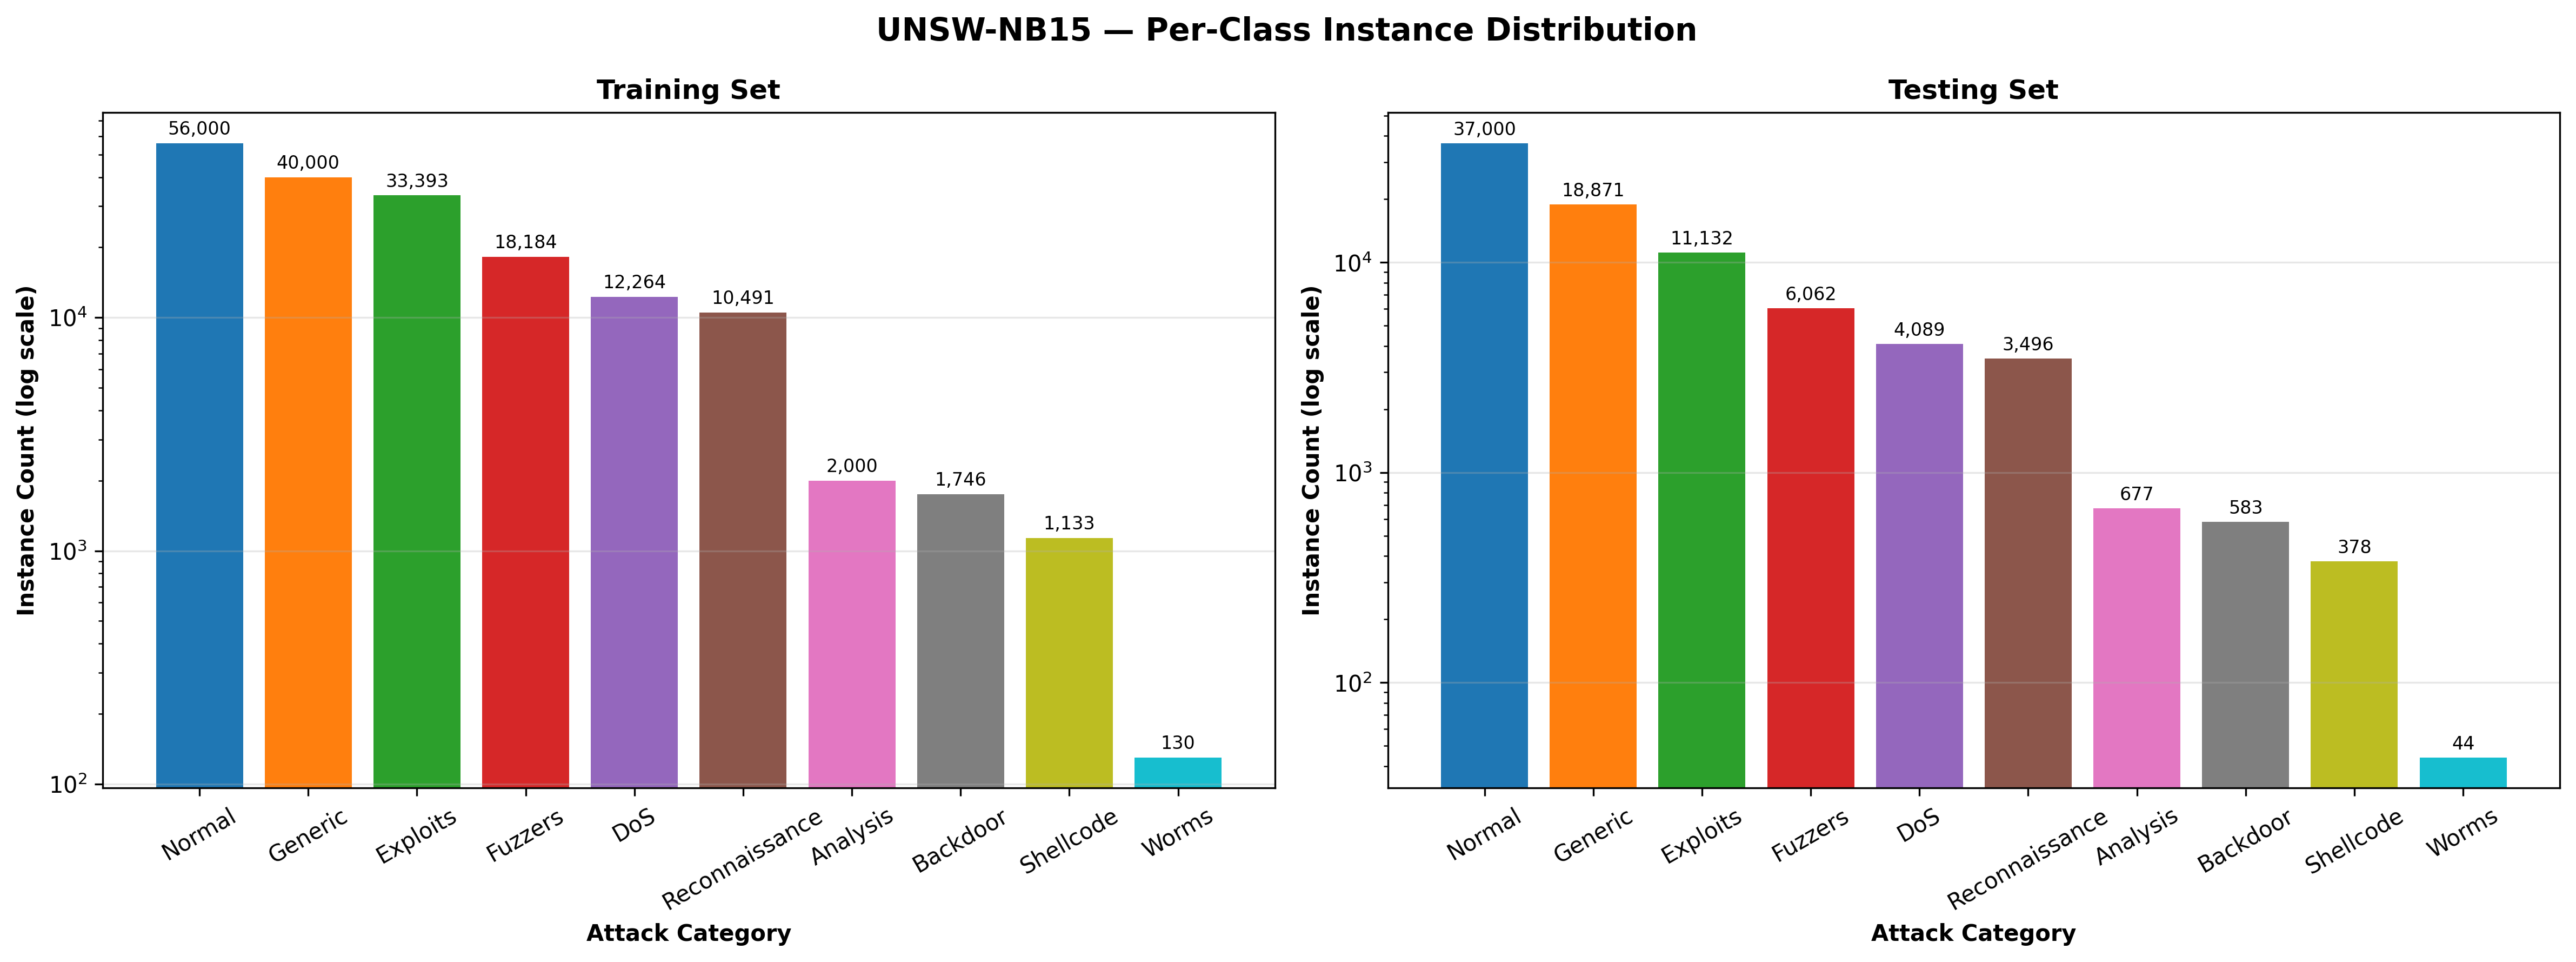
\includegraphics[width=\columnwidth]{class_distribution.png}
  \caption{Training set class distribution (175,341 instances, 10 classes).
           Log scale. Maximum imbalance ratio 430.77:1
           (Worms: 130; Normal: 56,000).}
  \label{fig:class_dist}
\end{figure}

\begin{figure}[t]
  \centering
  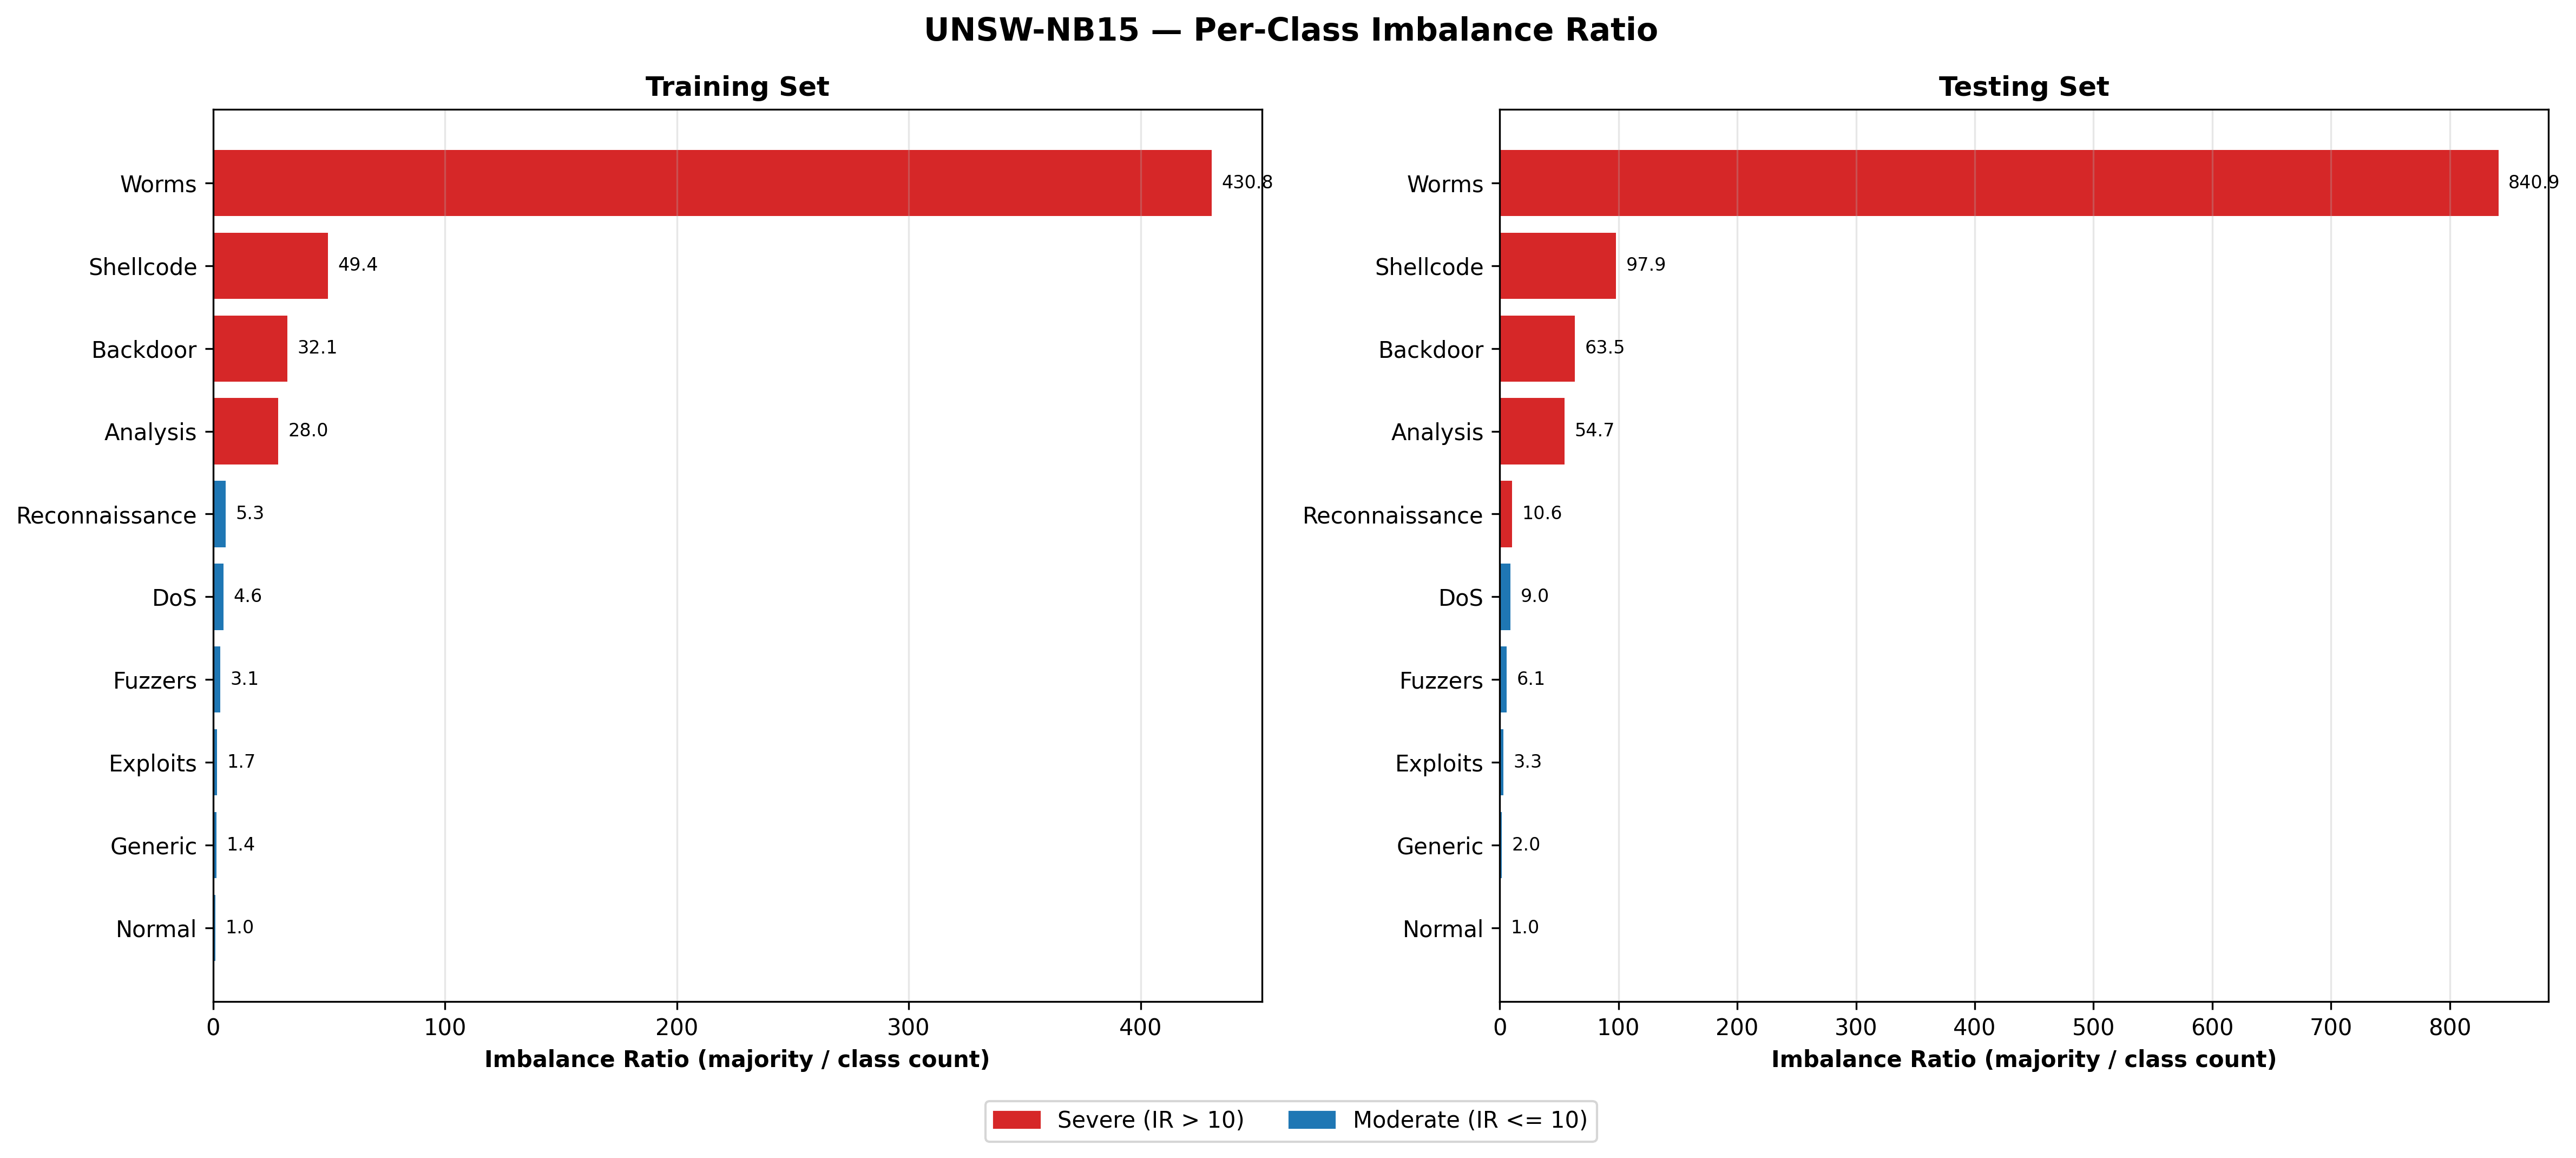
\includegraphics[width=\columnwidth]{imbalance_ratio.png}
  \caption{Per-class imbalance ratio relative to the Normal class
           (56,000 samples). Worms is the most severely underrepresented
           category (ratio 430.77:1).}
  \label{fig:imbalance}
\end{figure}

The UNSW-NB15 dataset \cite{moustafa2015} provides a predefined training set
(175,341 instances) and test set (82,332 instances) across 10 classes: Normal,
Analysis, Backdoor, DoS, Exploits, Fuzzers, Generic, Reconnaissance, Shellcode,
and Worms. The training set exhibits severe class imbalance: the Normal class
contains 56,000 samples (31.9\% of training), whereas Worms contains only 130
samples (0.074\%), yielding a maximum imbalance ratio of 430.77:1
(Fig.~\ref{fig:class_dist}, Fig.~\ref{fig:imbalance}).

\subsection{Feature Engineering and Preprocessing}

The original 44-feature schema was reduced to 42 features by removing \texttt{id}
(instance identifier; no discriminative value) and \texttt{label} (binary attack
indicator; target leakage). Numerical features were retained without additional
transformation; categorical features were encoded. No feature scaling was applied,
as Random Forest is scale-invariant.

\subsection{Class Rebalancing (SMOTE)}

\SMOTE \cite{chawla2002} was applied to the 42-feature training set with
\texttt{sampling\_strategy=`auto'} and \texttt{k\_neighbors=5}, using global
random seed~42. Minority classes were oversampled to match the majority-class
size (56,000 samples per class), producing a balanced training set of 560,000
rows (10 classes $\times$ 56,000 each). A total of 384,659 synthetic samples
were generated. The test set was not modified; both models are evaluated on the
same 82,332-row held-out set.

\subsection{Classifier}

A Random Forest \cite{breiman2001} classifier was trained independently on the
original imbalanced dataset (Baseline model) and on the \SMOTE-balanced dataset
(SMOTE model). All hyperparameters and the global random seed~(42) were held
constant between conditions. The original UNSW-NB15 train/test split was used
without re-splitting.

\subsection{XAI Methods}

\noindent\textbf{SHAP (TreeExplainer):} SHAP values \cite{lundberg2017,lundberg2020}
were computed for 60 test instances using \texttt{shap.TreeExplainer}, which
exploits the tree structure of Random Forest to compute exact Shapley values in
polynomial time. Global feature importance was obtained by averaging $|\text{SHAP}|$
values across instances. Feature rankings were compared between Baseline and SMOTE
models using Spearman rank correlation and top-5 overlap.

\smallskip
\noindent\textbf{LIME (LimeTabularExplainer):} LIME explanations \cite{ribeiro2016}
were computed for the same 60 instances using \texttt{LimeTabularExplainer} with
\texttt{num\_features=10} and \texttt{num\_samples=5000}. Each local explanation
is produced by a linear surrogate model fitted to perturbed samples in the instance
neighbourhood; the fidelity of this surrogate to the underlying Random Forest is
measured by the local coefficient of determination~($R^2$). Global importance was
derived by aggregating absolute LIME weights across instances.

\subsection{Statistical Validation}
\label{sec:stats}

Four hypothesis tests (Research Questions RQ1--RQ4) were conducted
(Table~\ref{tab:hyp}):
\begin{enumerate}
  \item \textbf{McNemar's test} (Yates continuity correction) on the 82,332-sample
        paired prediction matrix to assess whether the two models disagree at a
        statistically significant rate. McNemar's test is the appropriate paired
        test for comparing two classifiers on the same test set \cite{virtanen2020}.
        Discordant pairs: $b = 1{,}632$ (SMOTE gains), $c = 4{,}784$ (SMOTE losses).
  \item \textbf{Wilcoxon signed-rank test} on paired confidence scores (82,332
        pairs, normal approximation) to assess whether predicted class
        probabilities shifted. The Wilcoxon test was selected as a nonparametric
        alternative to a paired $t$-test, making no assumption of normality;
        34,002 pairs with zero difference were excluded using the Wilcoxon
        zero-method.
  \item \textbf{Wilcoxon signed-rank test} on paired SHAP global feature
        importances (42 feature pairs) to assess explanation magnitude shift.
  \item \textbf{Wilcoxon signed-rank test} on paired LIME global feature
        importances (36 feature pairs) to assess explanation magnitude shift.
\end{enumerate}

Holm--Bonferroni correction was applied across all four tests (adjusted
thresholds: $\alpha/4,\,\alpha/3,\,\alpha/2,\,\alpha$). Effect sizes are
reported using two complementary metrics. \cohensh quantifies the difference
between two proportions:
\begin{equation}
  h = 2\arcsin\!\sqrt{p_1} - 2\arcsin\!\sqrt{p_2},
  \label{eq:cohenh}
\end{equation}
where $|h|<0.20$ indicates a negligible effect, $\geq 0.20$ small,
$\geq 0.50$ medium, and $\geq 0.80$ large.
\rbs is derived from the Wilcoxon normal approximation:
\begin{equation}
  r = \frac{Z}{\sqrt{N}},
  \label{eq:rbs}
\end{equation}
where $N$ is the number of non-zero paired differences; $r\geq 0.10$ is
small, $\geq 0.30$ medium, and $\geq 0.50$ large (Cohen~1988 conventions
applied to both metrics). Because \cohensh operates on proportion data
($n=82{,}332$) and \rbs operates on feature importance ranks ($n=42$
or~36), these metrics are not on a common numerical scale; cross-metric
comparisons are interpreted as qualitative indicators of relative
sensitivity rather than precise proportional relationships.

Approximate statistical power for the Wilcoxon feature-importance tests: at
$n=42$ pairs with $r=0.326$ (SHAP), power $\approx 0.55$; at $n=36$ pairs
with $r=0.595$ (LIME), power $\approx 0.90$. The SHAP Wilcoxon result should
accordingly be interpreted as reaching significance at modest power.

Bootstrap confidence intervals (95\%, 2,000 resamples, percentile method) were
computed on the full 82,332-sample test set independently of the hypothesis tests.

% ==========================================================
\section{Experimental Setup}
\label{sec:setup}
% ==========================================================

All experiments were implemented in Python~3.10+. Key libraries include
scikit-learn \cite{pedregosa2011} for the Random Forest classifier and evaluation
metrics, imbalanced-learn \cite{lemaitre2017} for \SMOTE, \texttt{shap} \cite{lundberg2017}
for SHAP explanations, \texttt{lime} \cite{ribeiro2016} for LIME explanations,
SciPy \cite{virtanen2020} for statistical tests, and NumPy/pandas for numerical
computation. The global random seed was set to~42 for all stochastic operations
(\texttt{random}, \texttt{numpy}, scikit-learn).

SHAP and LIME explanations were computed on a stratified random sample of 60 test
instances (six instances per class), selected to balance computational tractability
with class-level coverage across all 10 categories. The identical set of 60
instances was used for both the Baseline and SMOTE models, ensuring that all
Baseline--SMOTE explanation comparisons are made on matched instance sets. This
deterministic shared-instance protocol eliminates instance-selection variance from
the paired comparison and improves reproducibility: given the same random seed and
sampling procedure, the 60-instance set is fully recoverable. Global feature
importances were derived by averaging absolute attribution values across these 60
instances. Statistical tests on feature importances used all 42 SHAP-retained and
36 LIME-retained feature pairs (features absent from one model's explanation set
were excluded from the paired comparison).

All configuration parameters (random seed, SMOTE hyperparameters, bootstrap
iteration count, significance levels) are stored in \texttt{configs/*.yaml} and
applied uniformly. All output artefacts are version-controlled via SHA-256 hashes
verified before statistical analysis. Full reproduction instructions are provided
in the repository.

% ==========================================================
\section{Results}
\label{sec:results}
% ==========================================================

\subsection{Predictive Performance (RQ1)}

\begin{figure}[t]
  \centering
  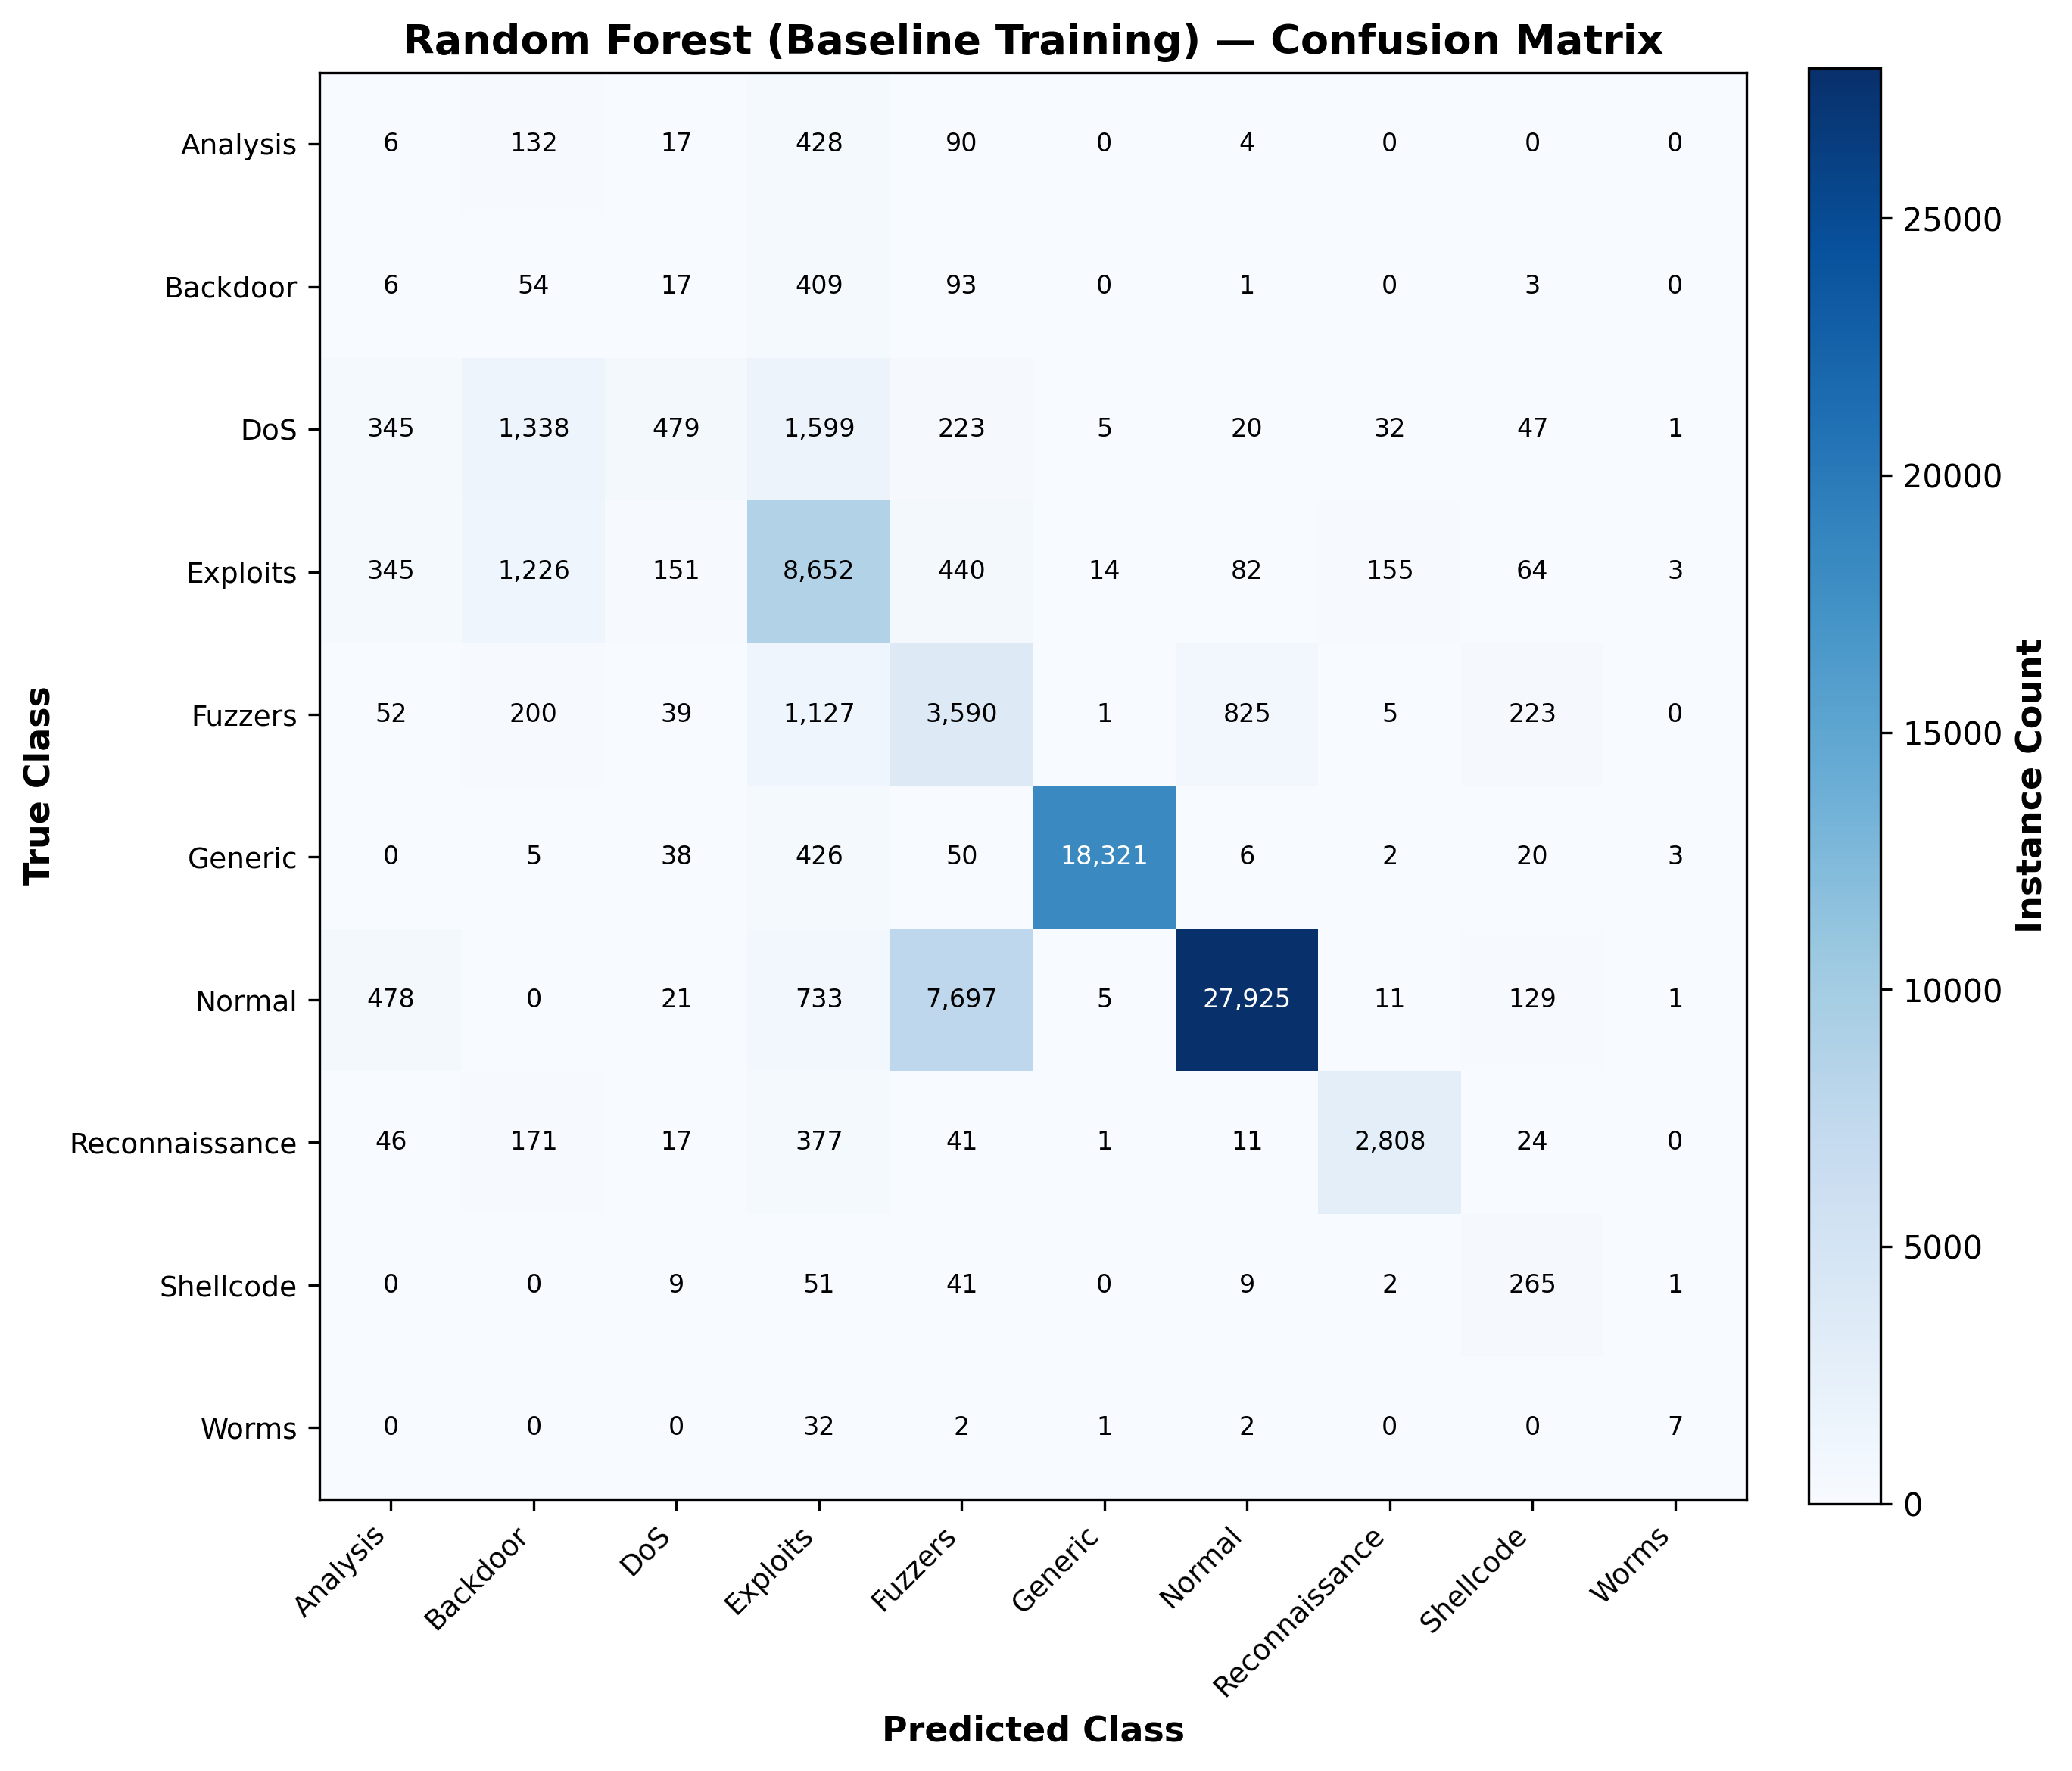
\includegraphics[width=\columnwidth]{confusion_matrix_baseline.png}
  \caption{Normalised confusion matrix --- Baseline model
           (test set, $n = 82{,}332$).}
  \label{fig:cm_base}
\end{figure}

\begin{figure}[t]
  \centering
  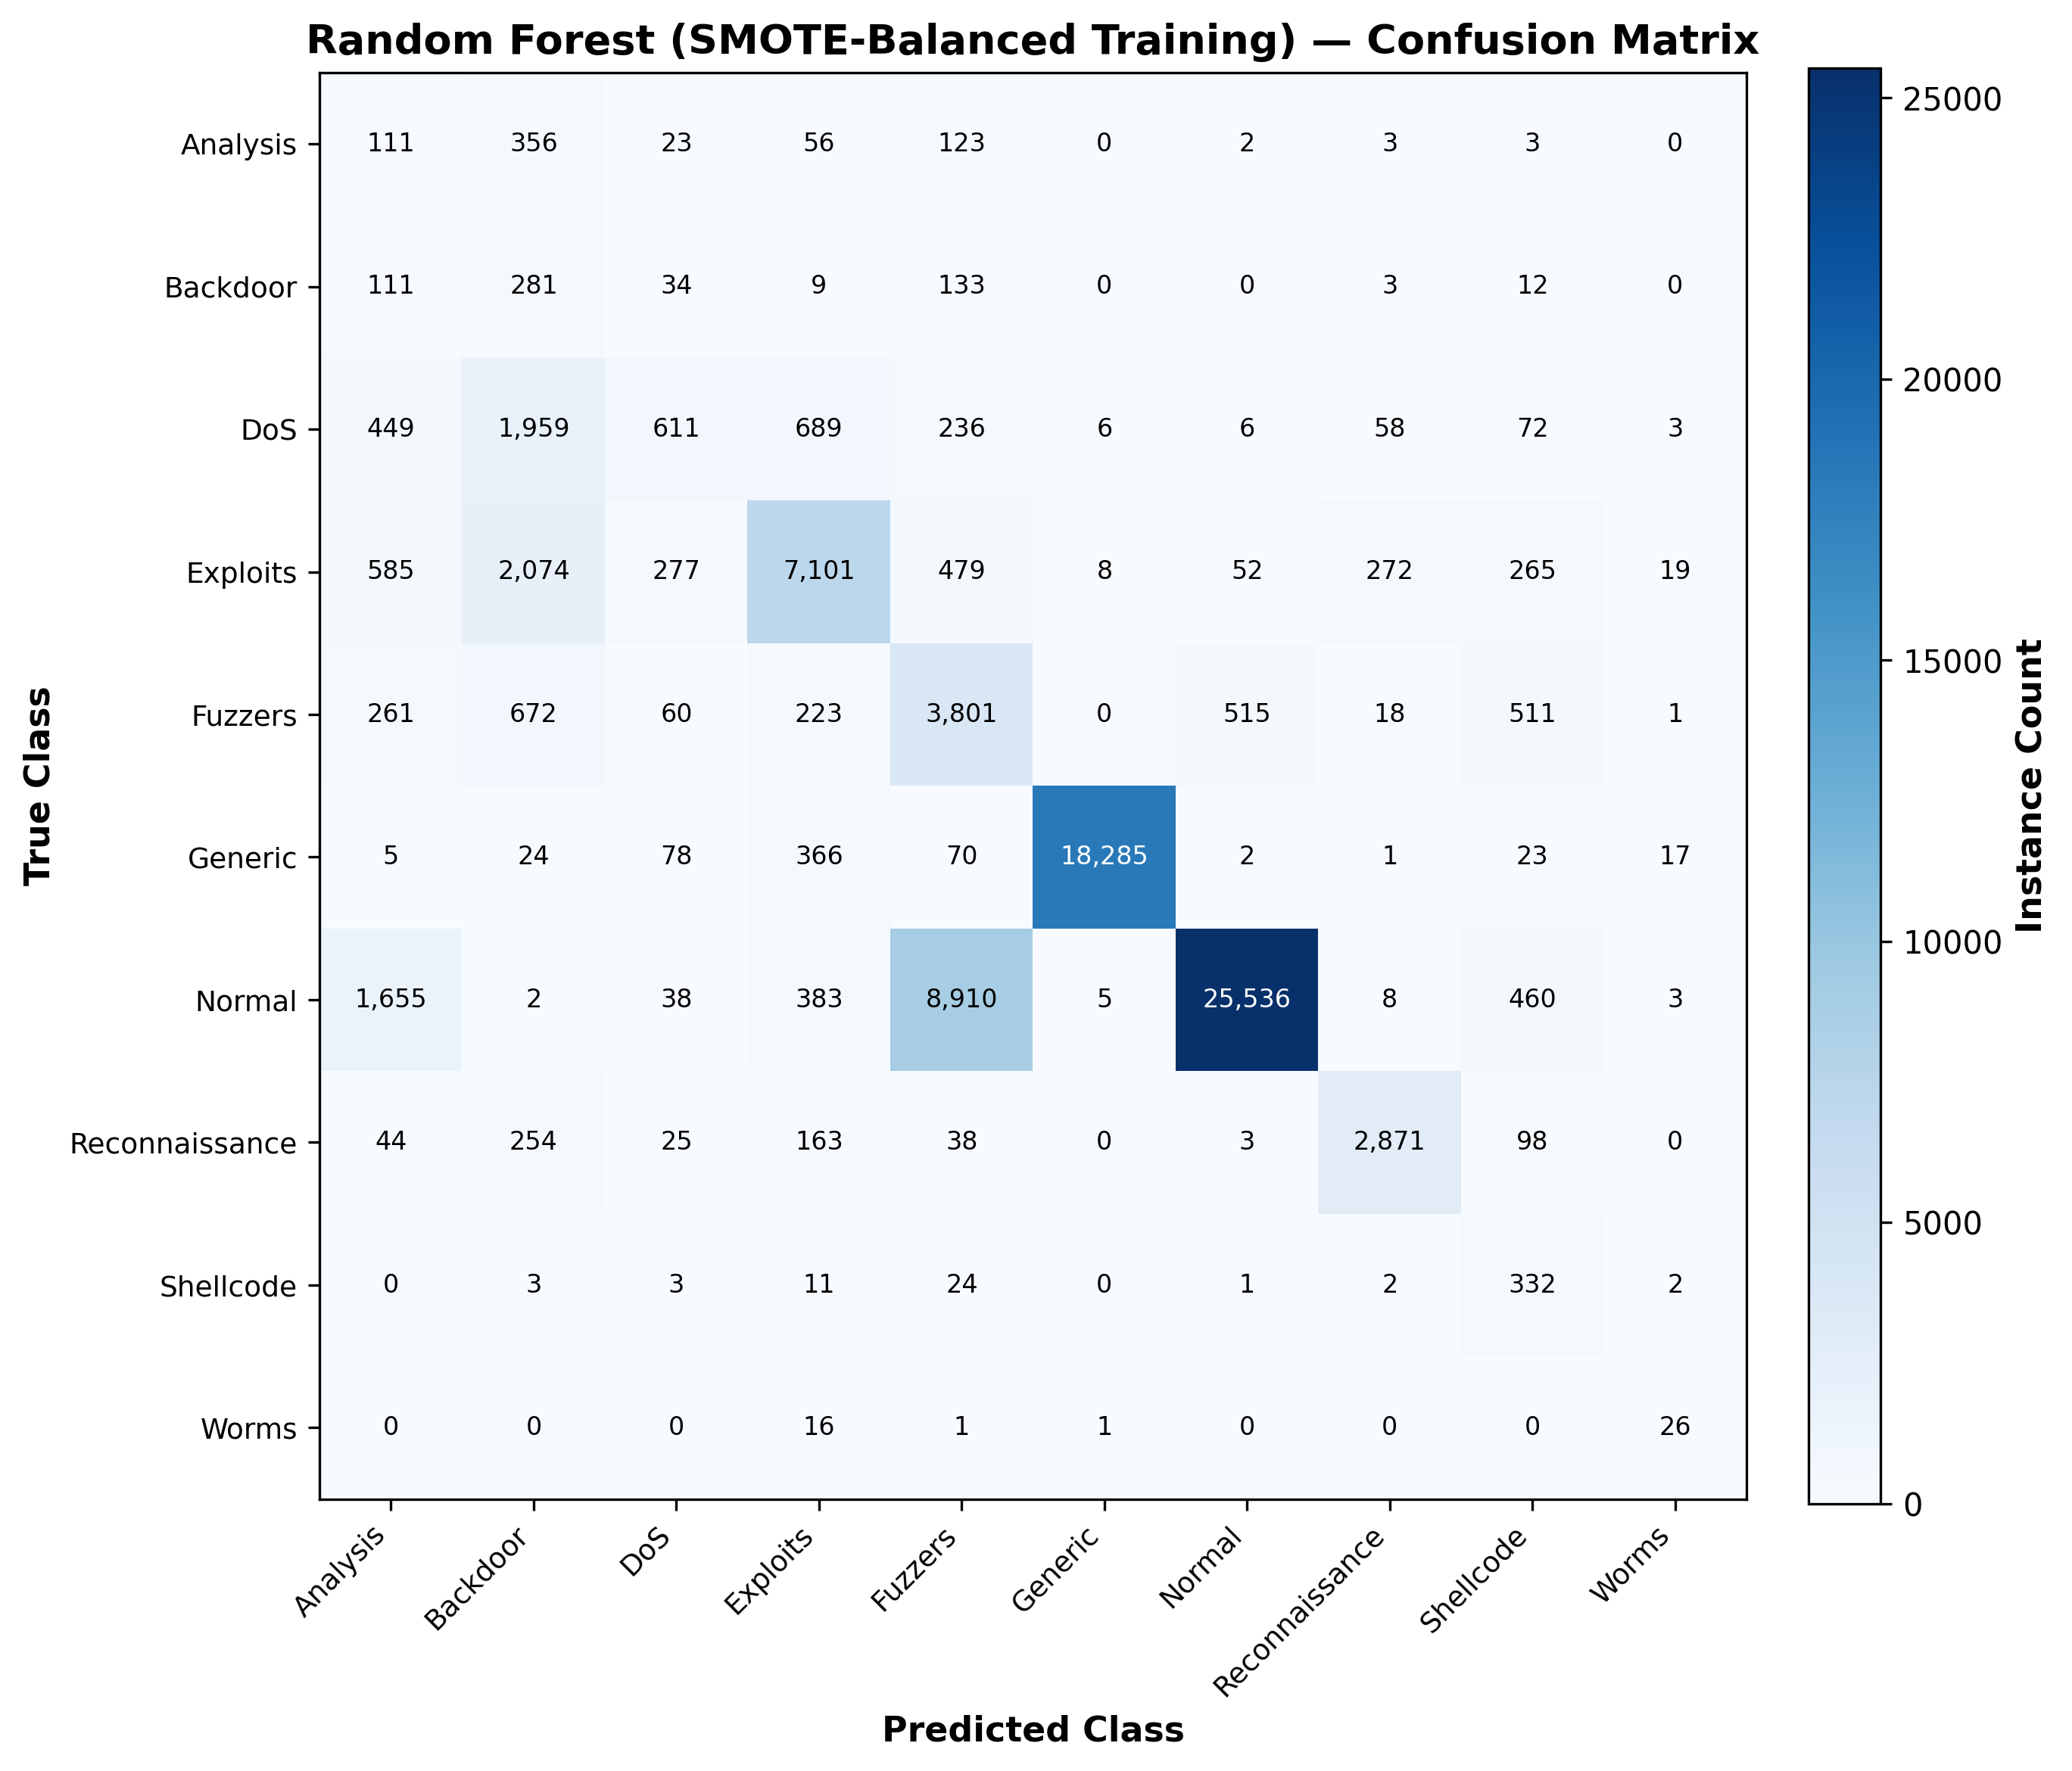
\includegraphics[width=\columnwidth]{confusion_matrix_smote.png}
  \caption{Normalised confusion matrix --- SMOTE model. Note improved
           Worms, Analysis, and Backdoor recall relative to
           Fig.~\ref{fig:cm_base}.}
  \label{fig:cm_smote}
\end{figure}

\begin{figure}[b]
  \centering
  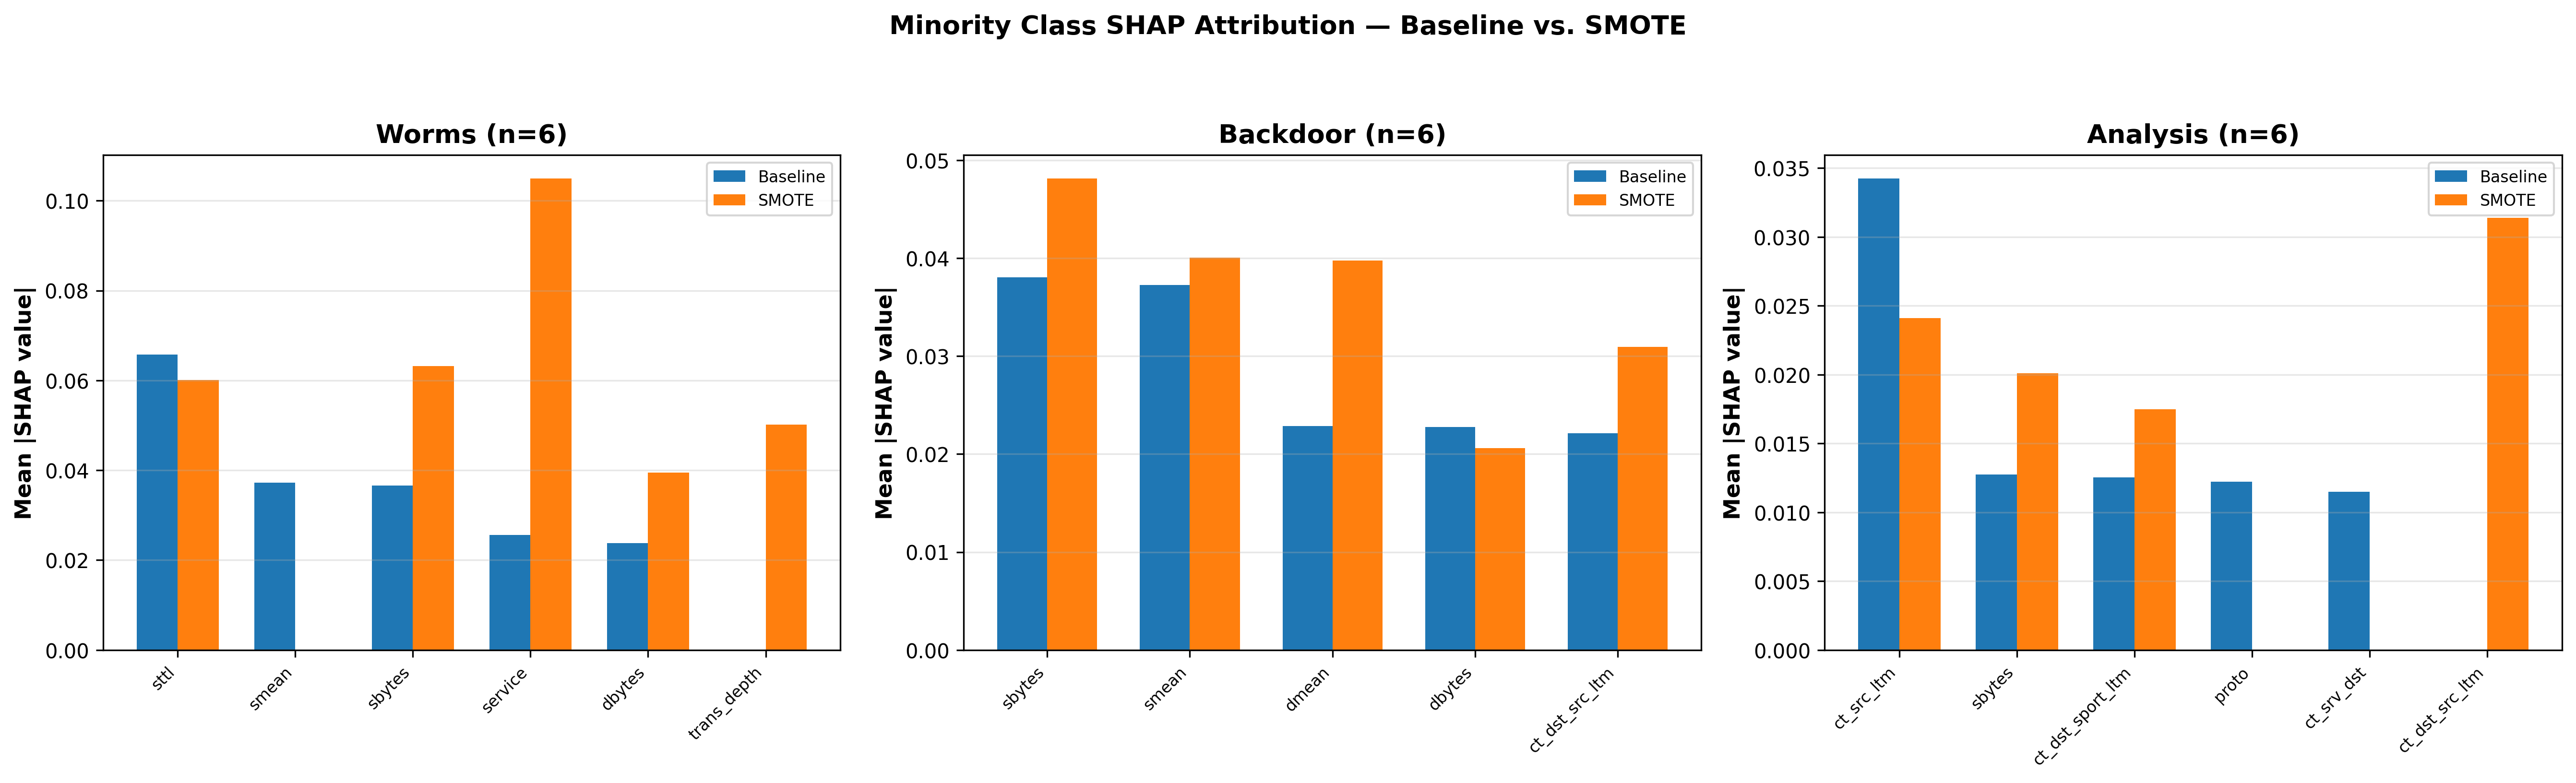
\includegraphics[width=\columnwidth]{minority_class_comparison.png}
  \caption{Per-class F1 score comparison: Baseline vs.\ SMOTE model.
           Minority classes (Analysis, Backdoor, Worms) gain; majority
           classes (Normal, Generic) decline marginally.}
  \label{fig:minority}
\end{figure}

Table~\ref{tab:perclass} reports per-class metrics for both models.
Table~\ref{tab:bootstrap} reports 95\% bootstrap confidence intervals for
aggregate metrics.

\SMOTE reduced accuracy by 0.0383 (0.7543 $\to$ 0.7161; 95\%~CI Baseline
$[0.7516,\,0.7574]$ vs.\ SMOTE $[0.7129,\,0.7191]$; non-overlapping) and weighted
F1 by 0.0149, while improving macro F1 by 0.0170 (95\%~CI Baseline
$[0.4556,\,0.4853]$ vs.\ SMOTE $[0.4752,\,0.4989]$).

McNemar's test confirmed that the models disagree at a statistically significant
rate ($\chi^2_{\text{Yates}}(1)=1547.51$, $p\approx 0$; corrected threshold
$\alpha=0.0125$). Of 82,332 test instances, 1,632 (1.98\%) were gained by \SMOTE
(Baseline wrong, SMOTE correct) while 4,784 (5.81\%) were lost. Despite
statistical significance, all \cohensh values are negligible:
$h(\text{accuracy})=-0.0868$, $h(\text{macro F1})=+0.0340$,
$h(\text{weighted F1})=-0.0354$ (Table~\ref{tab:effect}, Fig.~\ref{fig:effect}).

At the class level (Fig.~\ref{fig:cm_base}, Fig.~\ref{fig:cm_smote},
Fig.~\ref{fig:minority}, Table~\ref{tab:perclass}), \SMOTE improved F1 for
minority attack classes (mean recall gain $+0.325$ across minority categories;
Worms: $0.233\to0.452$) while degrading F1 for majority classes (mean F1
change $-0.020$; Normal: $0.848\to0.809$). This trade-off is the expected
consequence of synthetic oversampling: improved minority-class coverage at the
cost of majority-class precision.

The Worms test class contains only 44~instances; per-class F1 statistics at this
sample size are sensitive to individual prediction outcomes and are presented as
indicative results rather than stable estimates of population-level performance.

\smallskip
\noindent\textbf{Verdict (RQ1):} \SMOTE was partially beneficial --- statistically
significant aggregate differences but all negligible practical effect sizes;
minority-class F1 improved substantially while majority-class F1 declined modestly.

% --- TABLE I (full-width) ----------------------------------
\begin{table*}[t]
  \caption{Per-Class Classification Metrics --- Baseline and SMOTE Models
           (Test Set, $n = 82{,}332$)}
  \label{tab:perclass}
  \centering
  \begin{tabular}{lrrrrrrrr}
    \toprule
    \textbf{Class} &
      \textbf{P\,(B)} & \textbf{P\,(S)} &
      \textbf{R\,(B)} & \textbf{R\,(S)} &
      \textbf{F1\,(B)} & \textbf{F1\,(S)} &
      \bm{$n$} \\
    \midrule
    Analysis          & 0.005 & 0.034 & 0.009 & 0.164 & 0.006 & 0.057 & 677 \\
    Backdoor          & 0.017 & 0.050 & 0.093 & 0.482 & 0.029 & 0.091 & 583 \\
    DoS               & 0.608 & 0.532 & 0.117 & 0.149 & 0.196 & 0.233 & 4,089 \\
    Exploits          & 0.625 & 0.788 & 0.777 & 0.638 & 0.693 & 0.705 & 11,132 \\
    Fuzzers           & 0.293 & 0.275 & 0.592 & 0.627 & 0.392 & 0.382 & 6,062 \\
    Generic           & 0.999 & 0.999 & 0.971 & 0.969 & 0.984 & 0.984 & 18,871 \\
    Normal            & 0.967 & 0.978 & 0.755 & 0.690 & 0.848 & 0.809 & 37,000 \\
    Reconnaissance    & 0.931 & 0.887 & 0.803 & 0.821 & 0.863 & 0.853 & 3,496 \\
    Shellcode         & 0.342 & 0.187 & 0.701 & 0.878 & 0.460 & 0.308 & 378 \\
    Worms$^\dagger$   & 0.438 & 0.366 & 0.159 & 0.591 & 0.233 & 0.452 & 44 \\
    \midrule
    \textbf{Macro avg}    & 0.522 & 0.510 & 0.498 & 0.601 & 0.470 & 0.487 & 82,332 \\
    \textbf{Weighted avg} & 0.826 & 0.836 & 0.754 & 0.716 & 0.778 & 0.763 & 82,332 \\
    \bottomrule
    \multicolumn{8}{l}{\footnotesize B = Baseline; S = SMOTE;
      P = Precision; R = Recall; F1 = F1-score. Values rounded to 3 d.p.}\\
    \multicolumn{8}{l}{\footnotesize $^\dagger$ $n=44$; metrics indicative only
      (see Section~\ref{sec:results}-A).}\\
  \end{tabular}
\end{table*}

% --- TABLE II ----------------------------------------------
\begin{table}[t]
  \caption{Bootstrap 95\% Confidence Intervals for Aggregate Metrics
           ($n_{\text{resample}} = 2{,}000$, Percentile Method)}
  \label{tab:bootstrap}
  \centering
  \begin{tabular}{llrrrr}
    \toprule
    \textbf{Model} & \textbf{Metric} &
      \textbf{Obs.} & \textbf{CI$_\text{lo}$} & \textbf{CI$_\text{hi}$} &
      \textbf{Width} \\
    \midrule
    Baseline & Accuracy    & 0.7543 & 0.7516 & 0.7574 & 0.0057 \\
    Baseline & Macro F1    & 0.4704 & 0.4556 & 0.4853 & 0.0298 \\
    Baseline & Weighted F1 & 0.7780 & 0.7754 & 0.7808 & 0.0054 \\
    SMOTE    & Accuracy    & 0.7161 & 0.7129 & 0.7191 & 0.0062 \\
    SMOTE    & Macro F1    & 0.4874 & 0.4752 & 0.4989 & 0.0237 \\
    SMOTE    & Weighted F1 & 0.7631 & 0.7605 & 0.7659 & 0.0054 \\
    \bottomrule
    \multicolumn{6}{l}{\footnotesize Non-overlapping accuracy CIs corroborate
      McNemar's test.}\\
  \end{tabular}
\end{table}

% ----------------------------------------------------------
\subsection{Explanation Quality (RQ2)}

\begin{figure}[t]
  \centering
  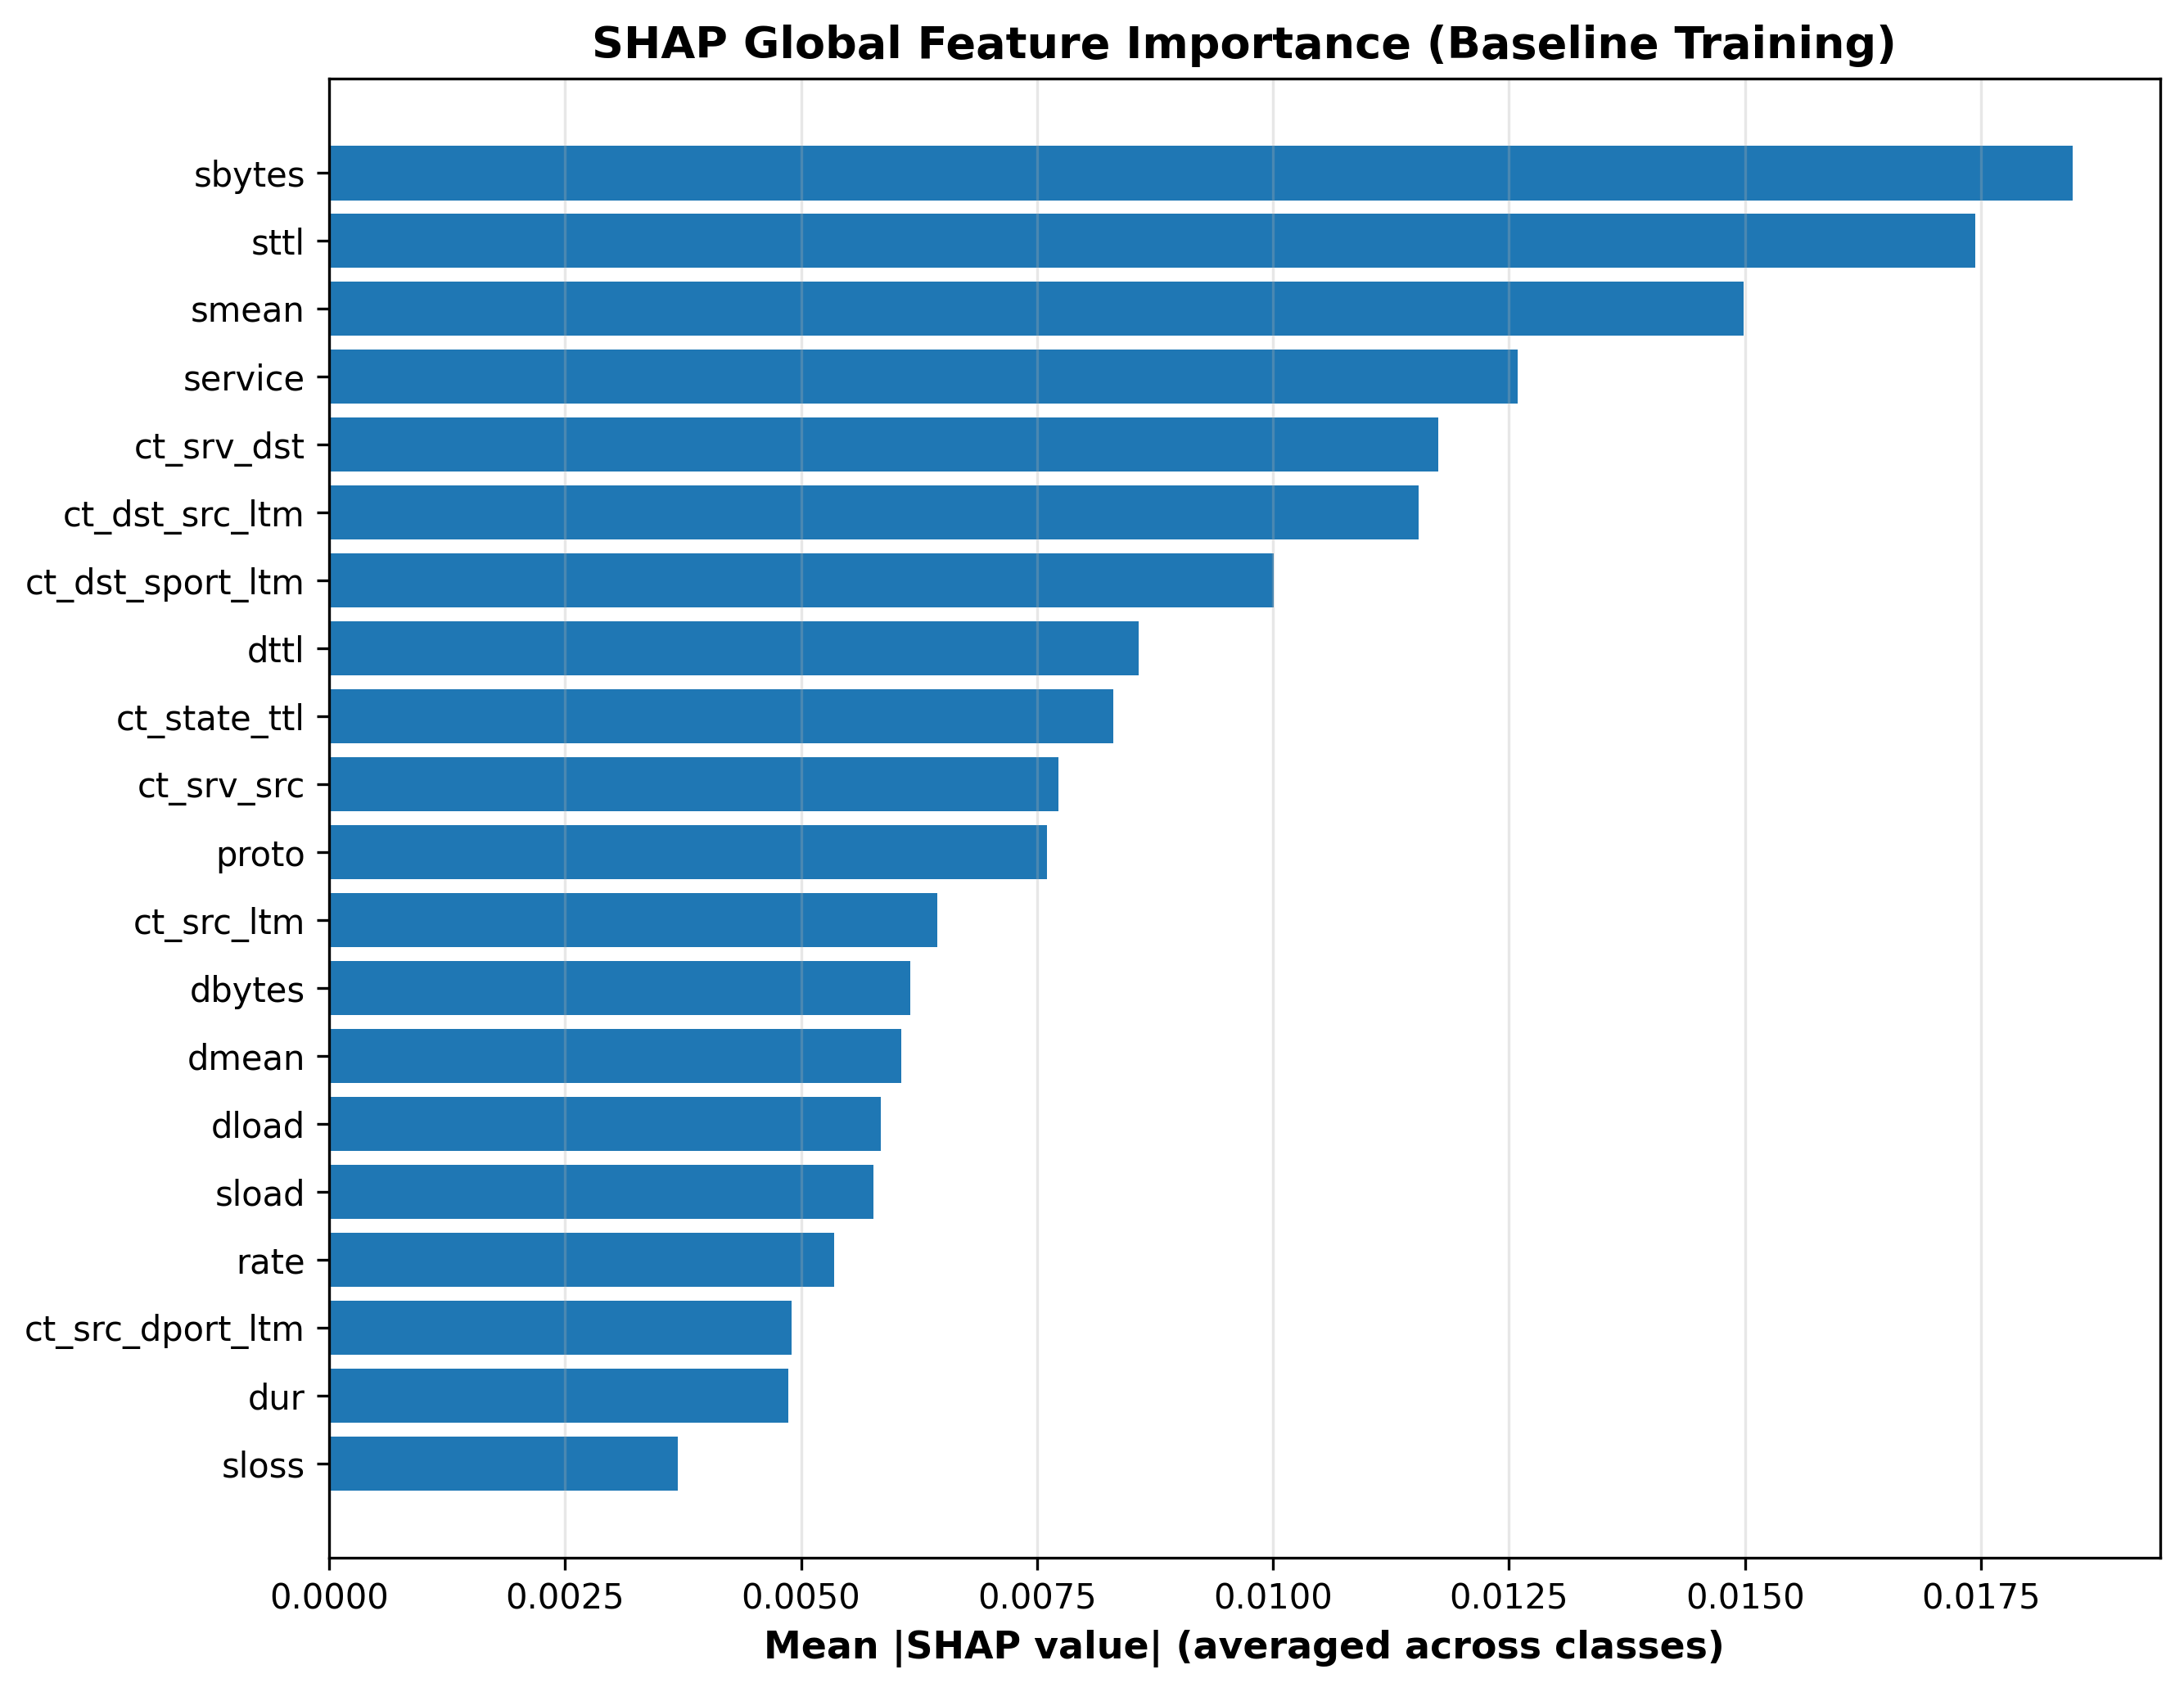
\includegraphics[width=\columnwidth]{shap_bar_baseline.png}
  \caption{SHAP global feature importance --- Baseline model
           (mean $|\text{SHAP value}|$ over 60 instances $\times$ 10 classes).
           Top feature: \texttt{sbytes} (0.0185).}
  \label{fig:shap_base}
\end{figure}

\begin{figure}[t]
  \centering
  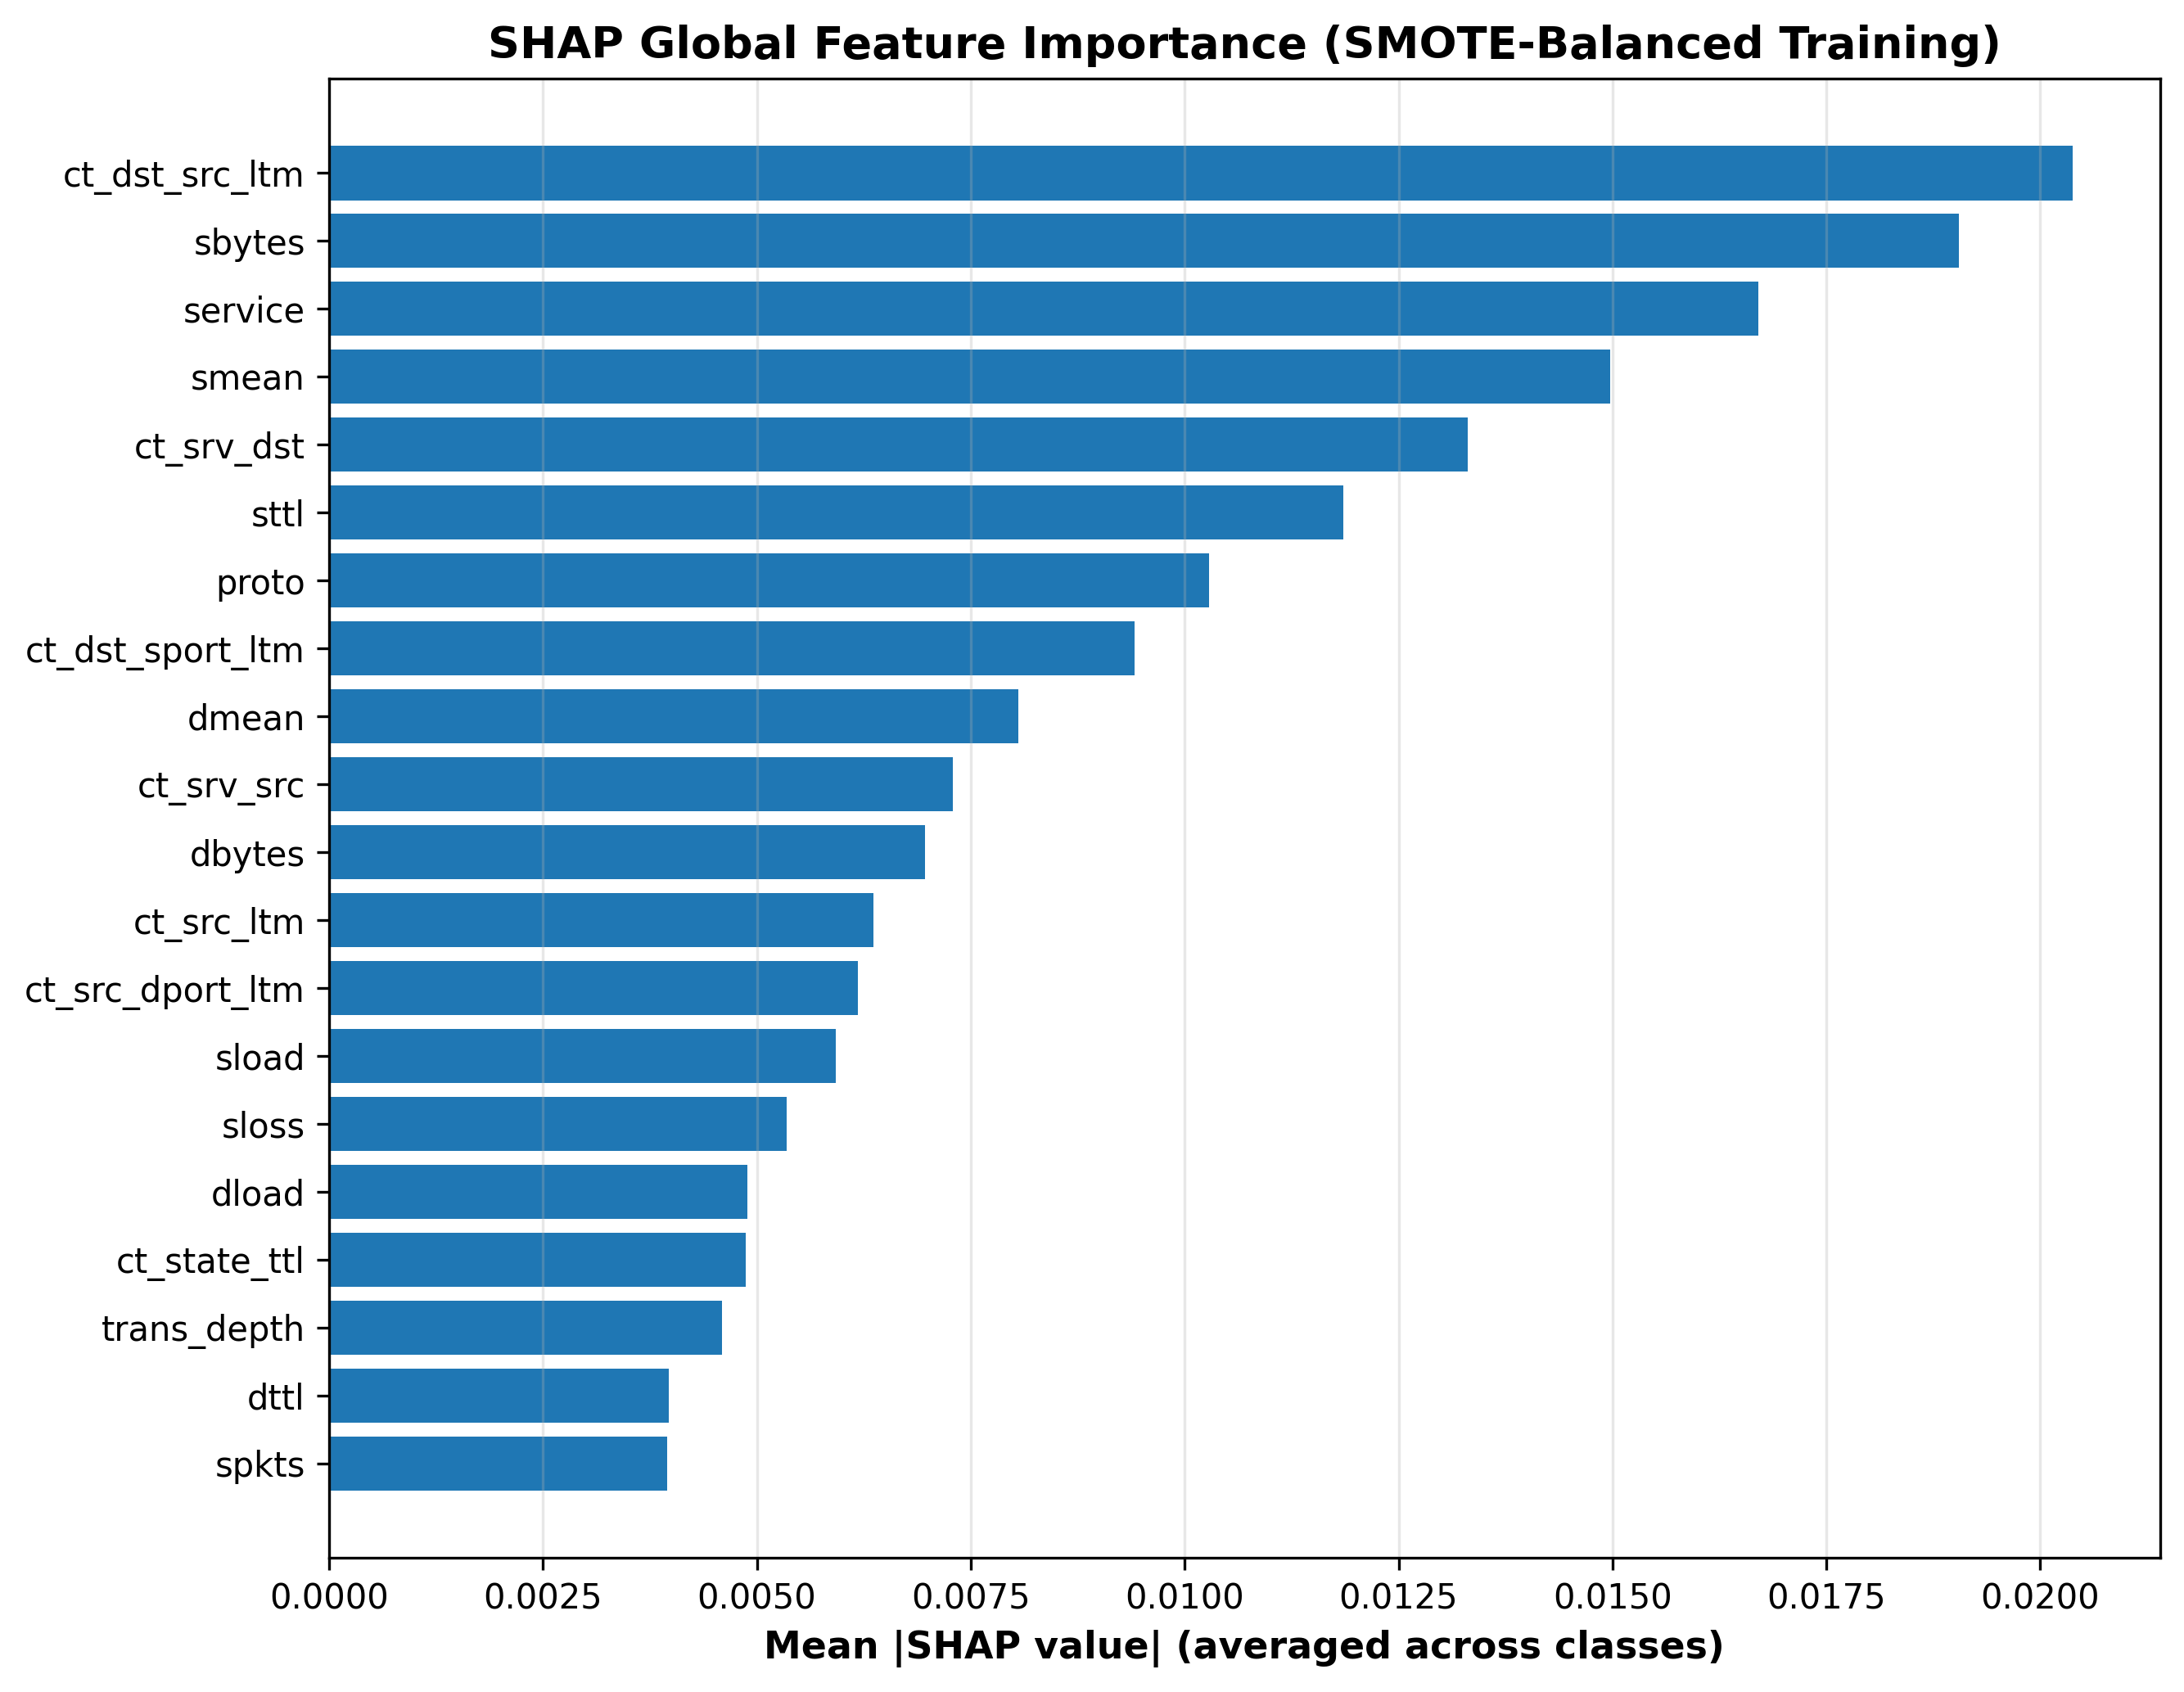
\includegraphics[width=\columnwidth]{shap_bar_smote.png}
  \caption{SHAP global feature importance --- SMOTE model.
           Top feature: \texttt{ct\_dst\_src\_ltm} (0.0204).
           Spearman $\rho=0.900$ vs.\ Fig.~\ref{fig:shap_base};
           top-5 overlap $=0.80$.}
  \label{fig:shap_smote}
\end{figure}

\begin{figure}[b]
  \centering
  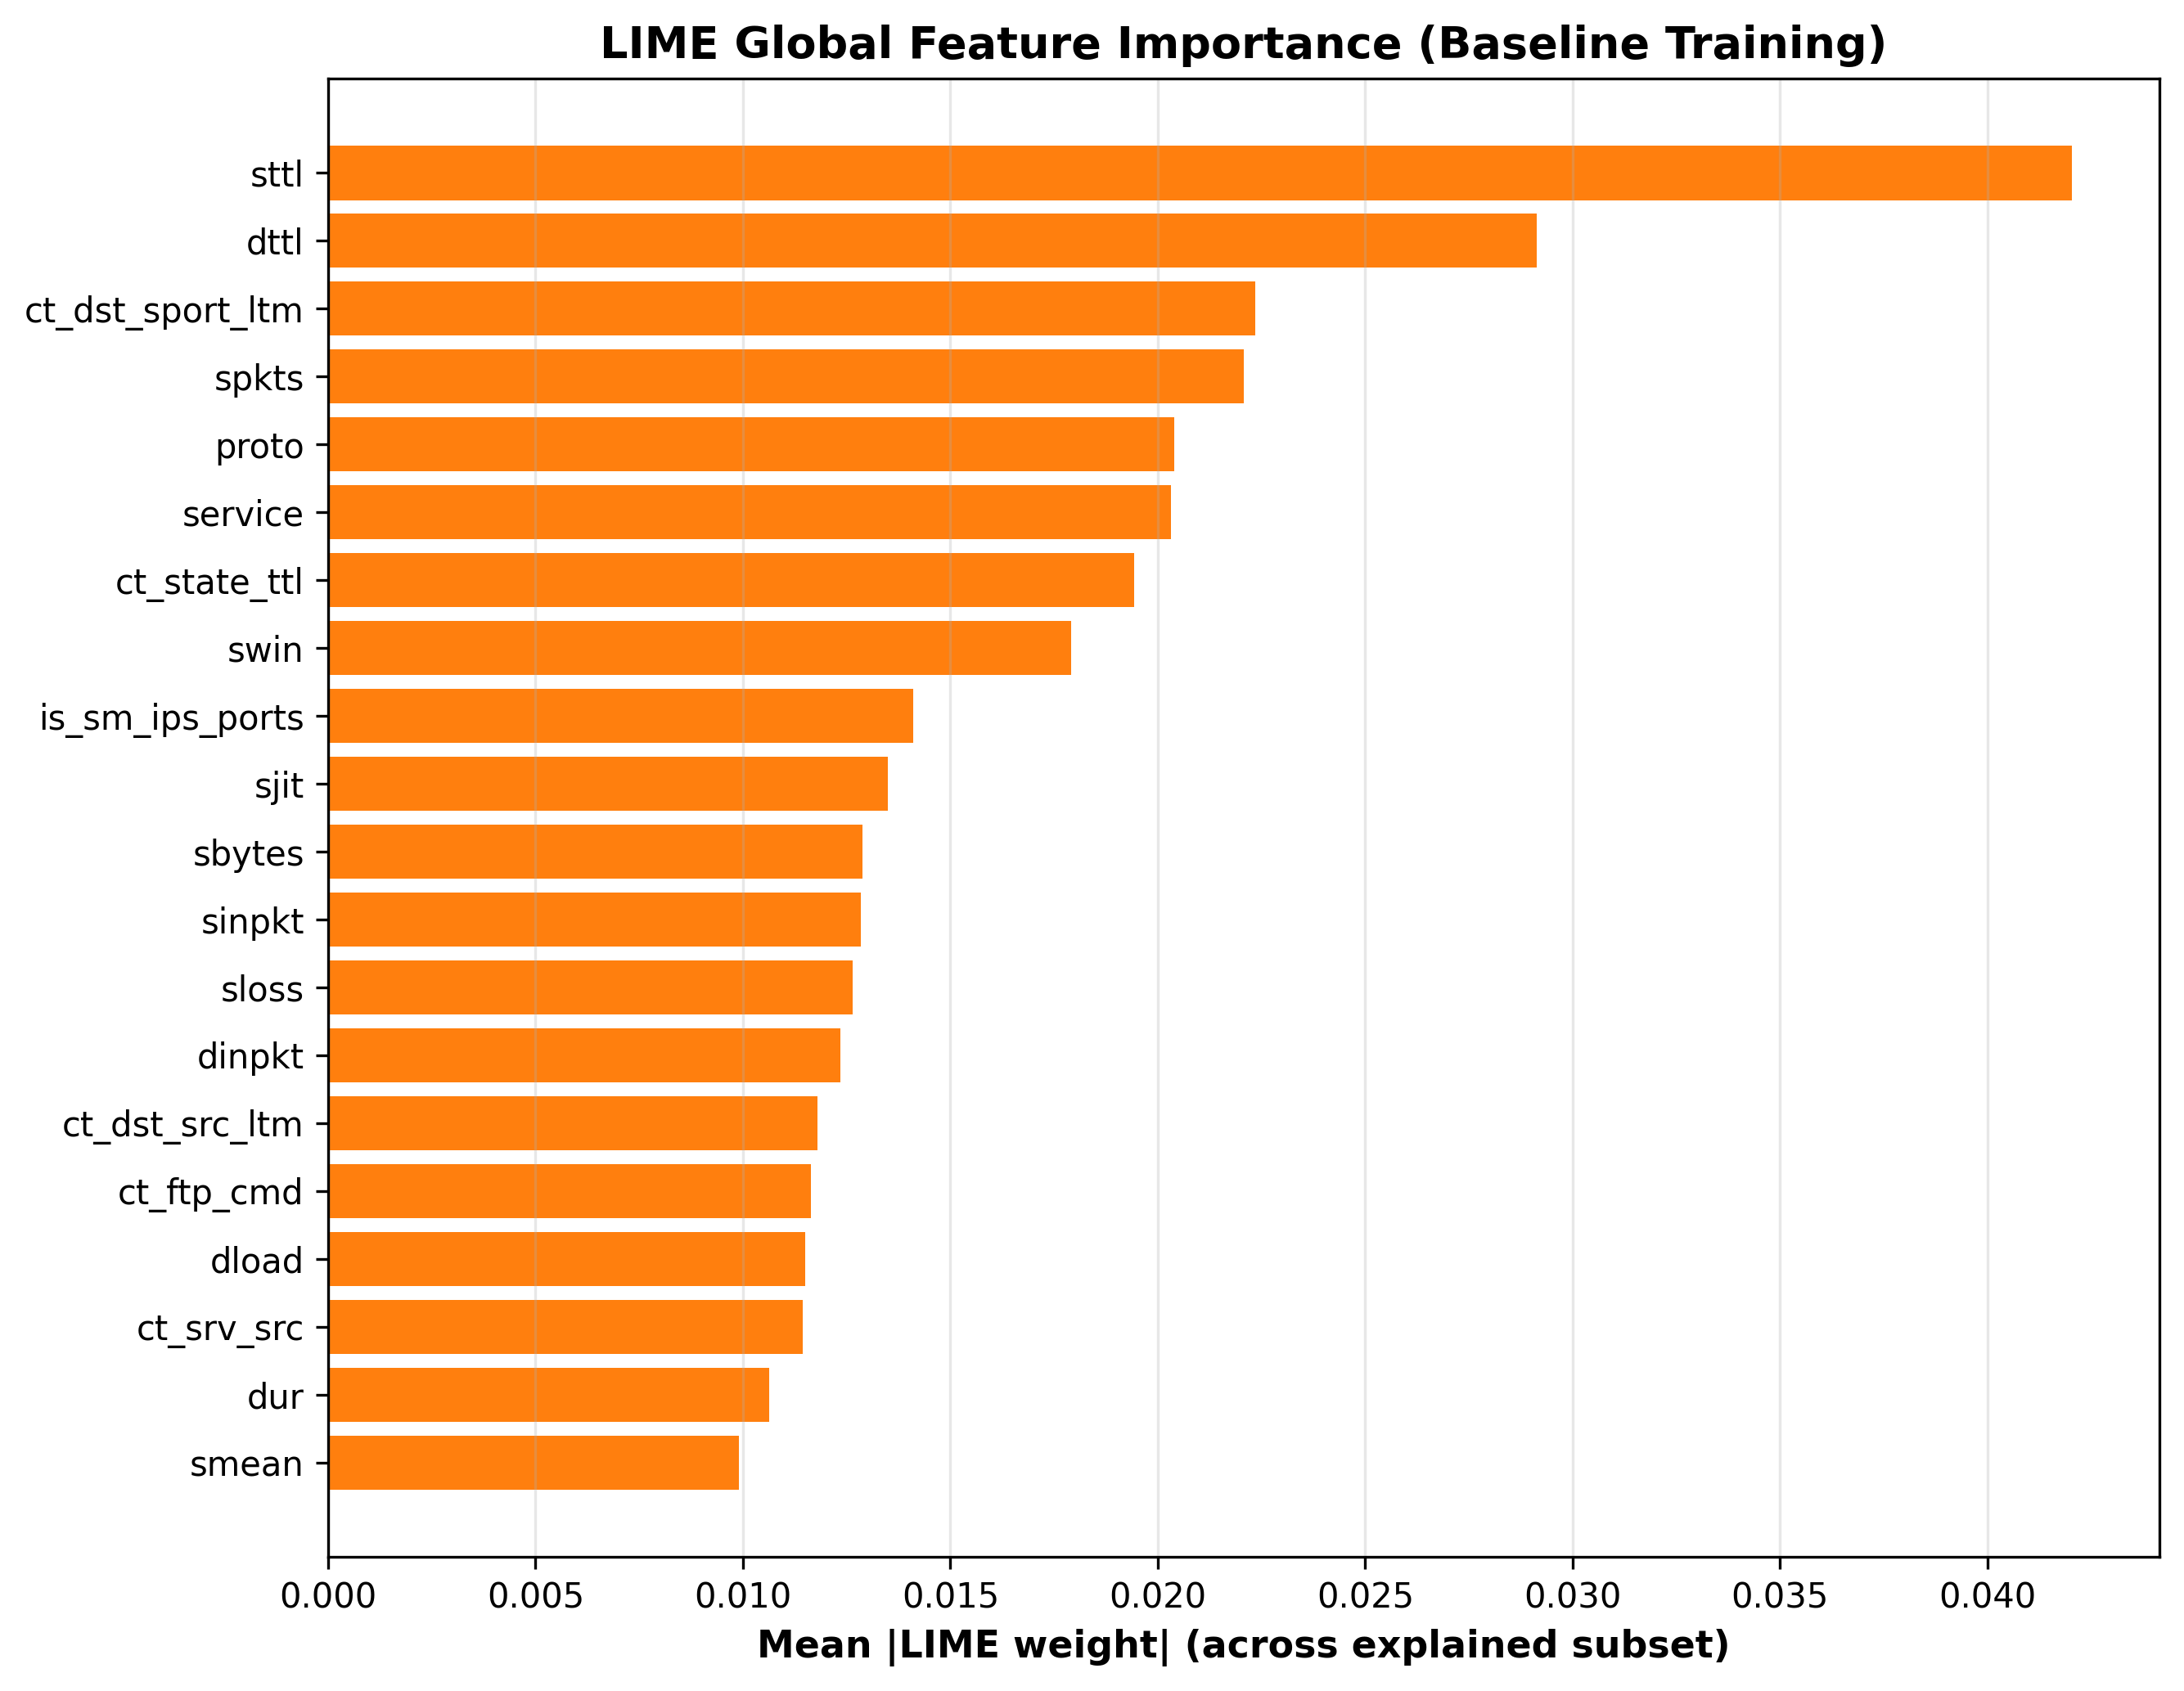
\includegraphics[width=\columnwidth]{lime_importance_baseline.png}
  \caption{LIME global feature importance --- Baseline model
           (mean $|\text{weight}|$ over 60 instances).
           Top feature: \texttt{sttl} (0.042; 53/60 appearances).
           Mean local $R^2 = 0.290$.}
  \label{fig:lime_base}
\end{figure}

\begin{figure}[b]
  \centering
  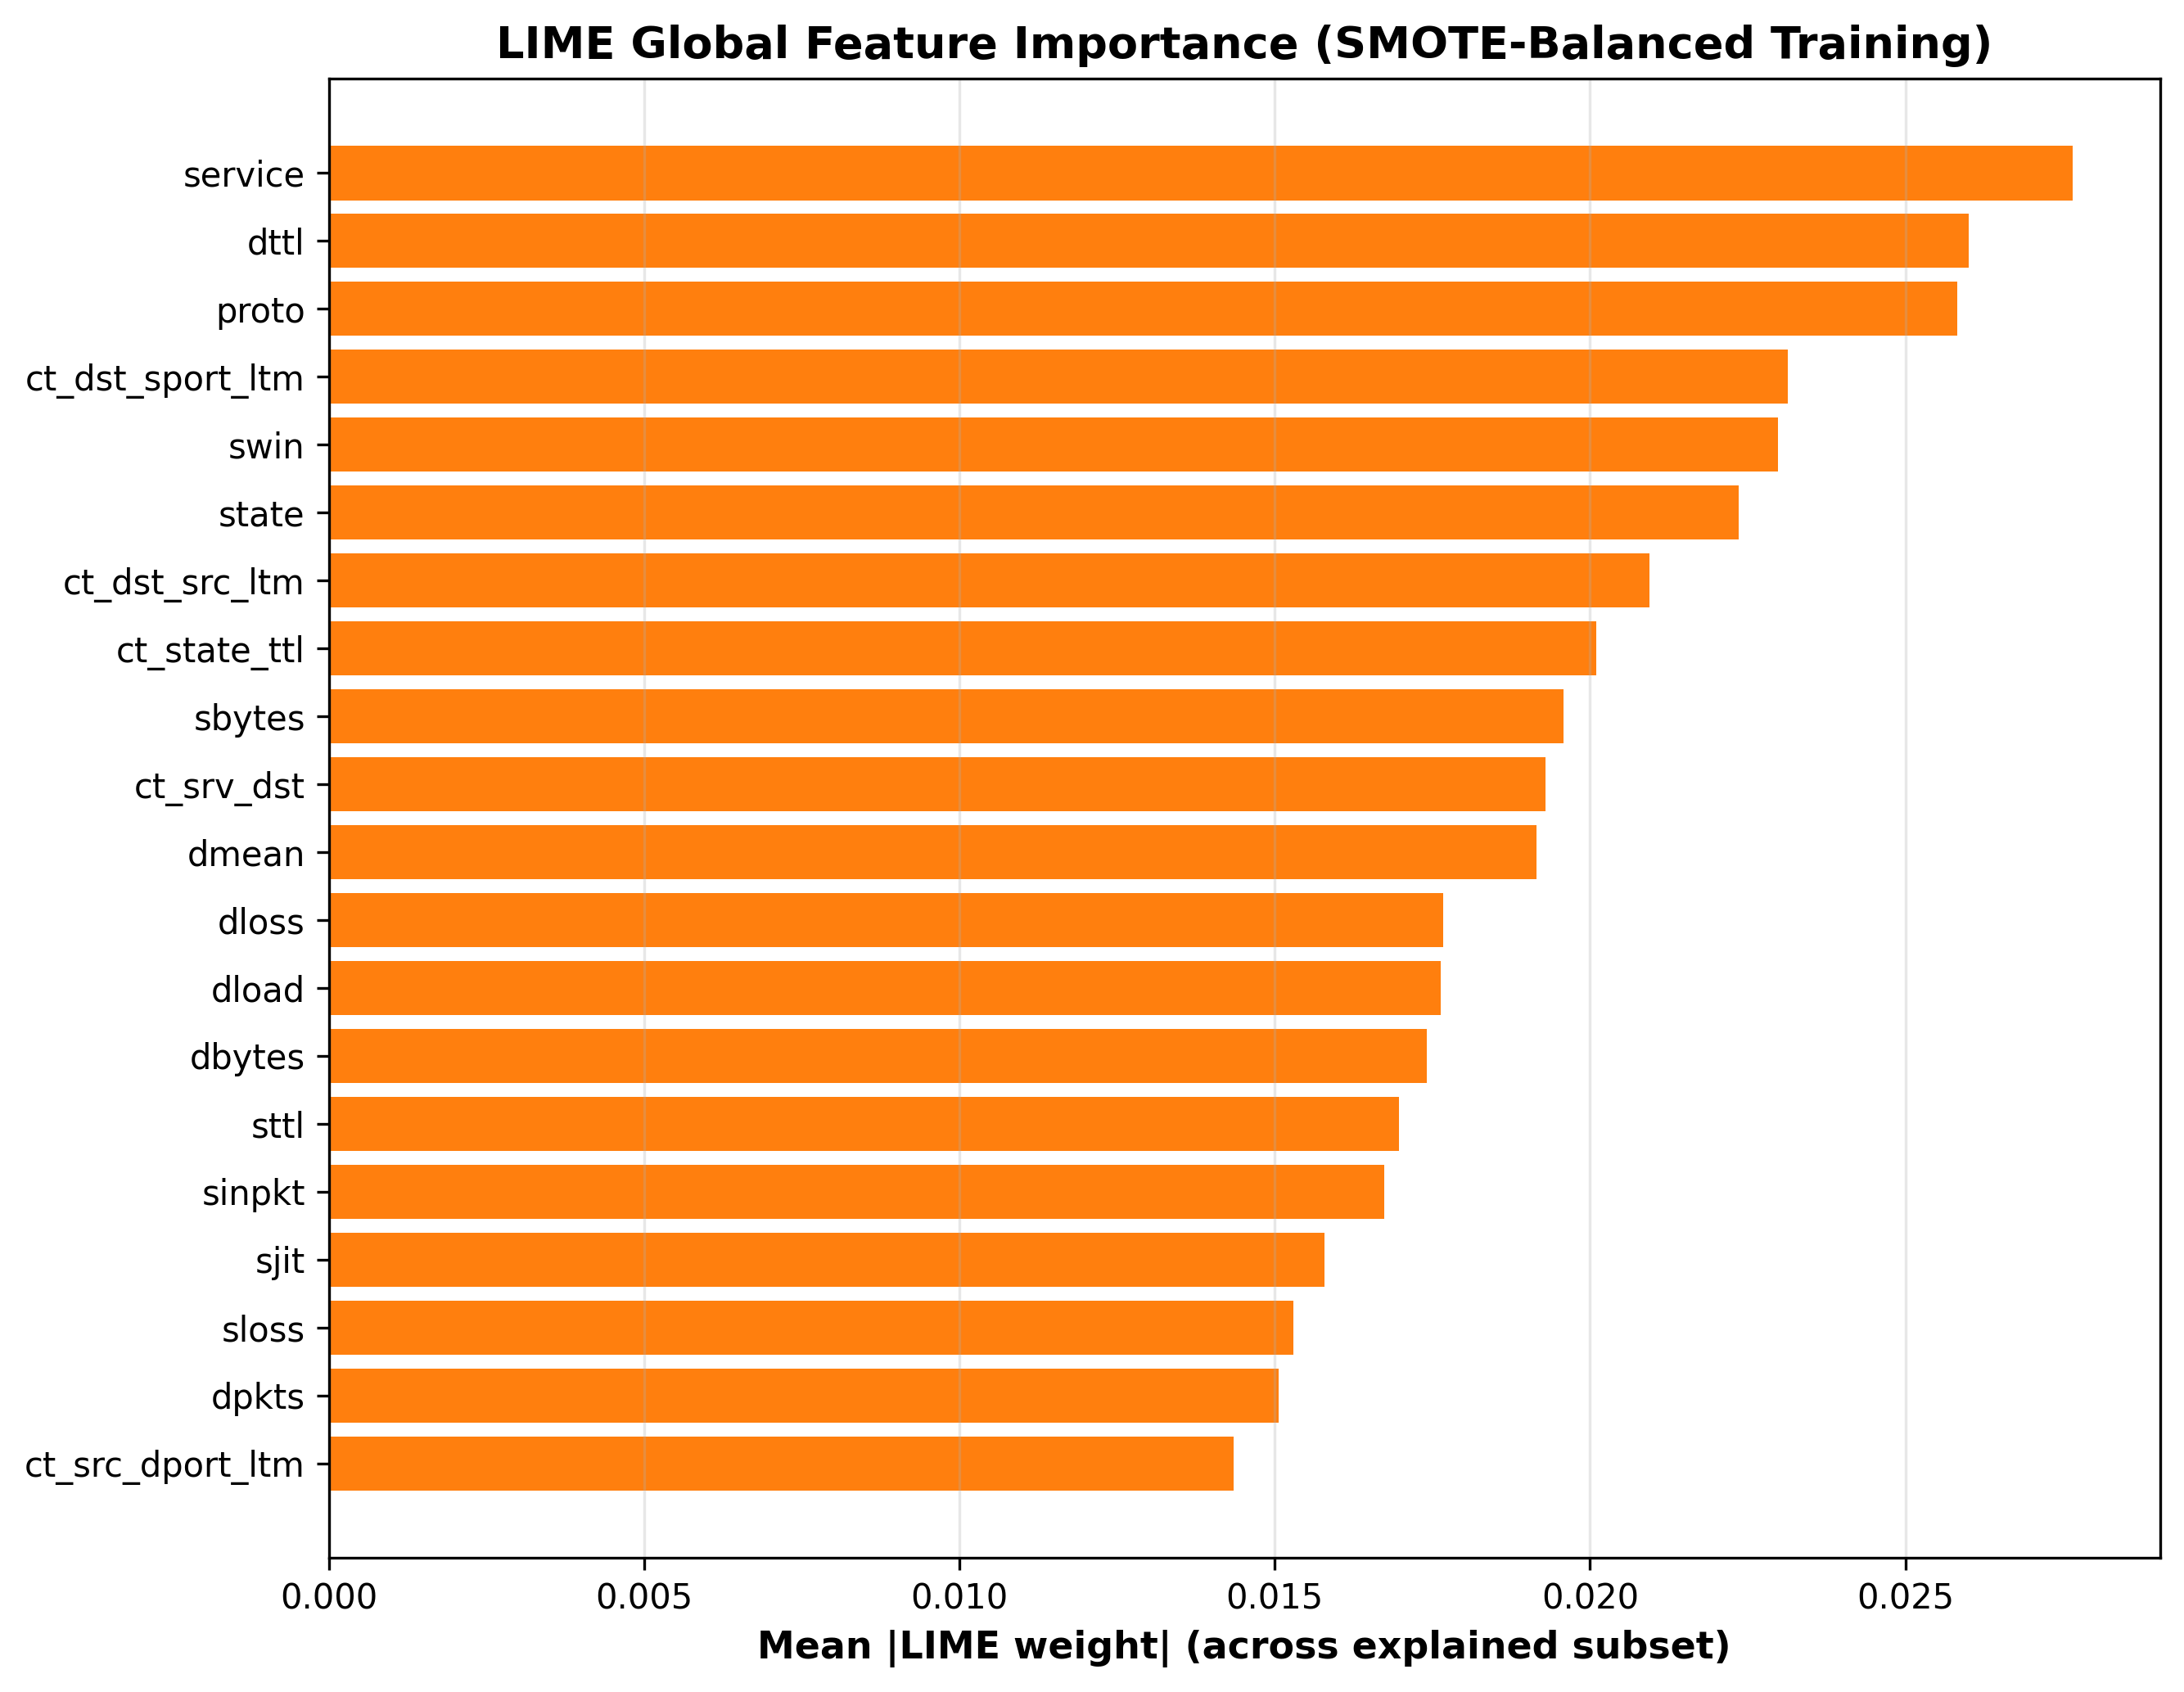
\includegraphics[width=\columnwidth]{lime_importance_smote.png}
  \caption{LIME global feature importance --- SMOTE model.
           Top feature: \texttt{service} (0.028; 60/60 appearances).
           Spearman $\rho=0.565$ vs.\ Fig.~\ref{fig:lime_base};
           top-5 overlap $=0.60$. Mean local $R^2 = 0.252$.}
  \label{fig:lime_smote}
\end{figure}

SHAP global feature attribution rankings showed moderate stability across
conditions (Spearman $\rho=0.900$, top-5 overlap $=0.80$)
(Fig.~\ref{fig:shap_base}, Fig.~\ref{fig:shap_smote}, Fig.~\ref{fig:ranking}).
A Wilcoxon signed-rank test on 42 paired feature importances confirmed a
statistically significant distributional shift ($W=283$, $p=0.0347$;
Holm-corrected threshold $\alpha=0.050$) with a medium practical effect
(rank-biserial $r=0.3259$) (Table~\ref{tab:hyp}, Fig.~\ref{fig:effect}).

LIME global feature attribution rankings showed considerably lower stability
(Spearman $\rho=0.565$, top-5 overlap $=0.60$)
(Fig.~\ref{fig:lime_base}, Fig.~\ref{fig:lime_smote}, Fig.~\ref{fig:ranking}).
The Wilcoxon test on 36 paired LIME importances confirmed a larger and more
significant shift ($W=115$, $p=3.59\times10^{-4}$; Holm-corrected threshold
$\alpha=0.025$) with a large practical effect ($r=0.5947$)
(Table~\ref{tab:hyp}).

LIME local surrogate fidelity, measured by the mean $R^2$ of each instance's
local linear model, was 0.290 for the Baseline model and 0.252 for the SMOTE
model (Fig.~\ref{fig:lime_base}, Fig.~\ref{fig:lime_smote}). These values
indicate that the local surrogate captures approximately 25--29\% of the Random
Forest's local decision variance. The observed shift in LIME attribution rankings
is statistically robust; however, LIME attribution magnitudes reflect the linear
surrogate under moderate fidelity conditions and should be understood as
approximations of local model behaviour rather than exact attributions.

Inter-method agreement between SHAP and LIME was low in both conditions
(Spearman $\rho=0.410$ at Baseline, $\rho=0.476$ after SMOTE), consistent
with SHAP and LIME capturing different aspects of model behaviour. \SMOTE
slightly improved inter-method agreement.

\smallskip
\noindent\textbf{Verdict (RQ2):} \SMOTE caused a statistically significant change
in \XAI explanations; LIME attribution rankings exhibited a larger shift than
SHAP (large vs.\ medium effect), with LIME results interpreted in light of
moderate local surrogate fidelity ($R^2\approx 0.25$--$0.29$).

% ----------------------------------------------------------
\subsection{Predictive vs.\ Explanatory Sensitivity (RQ3)}

\begin{figure*}[t]
  \centering
  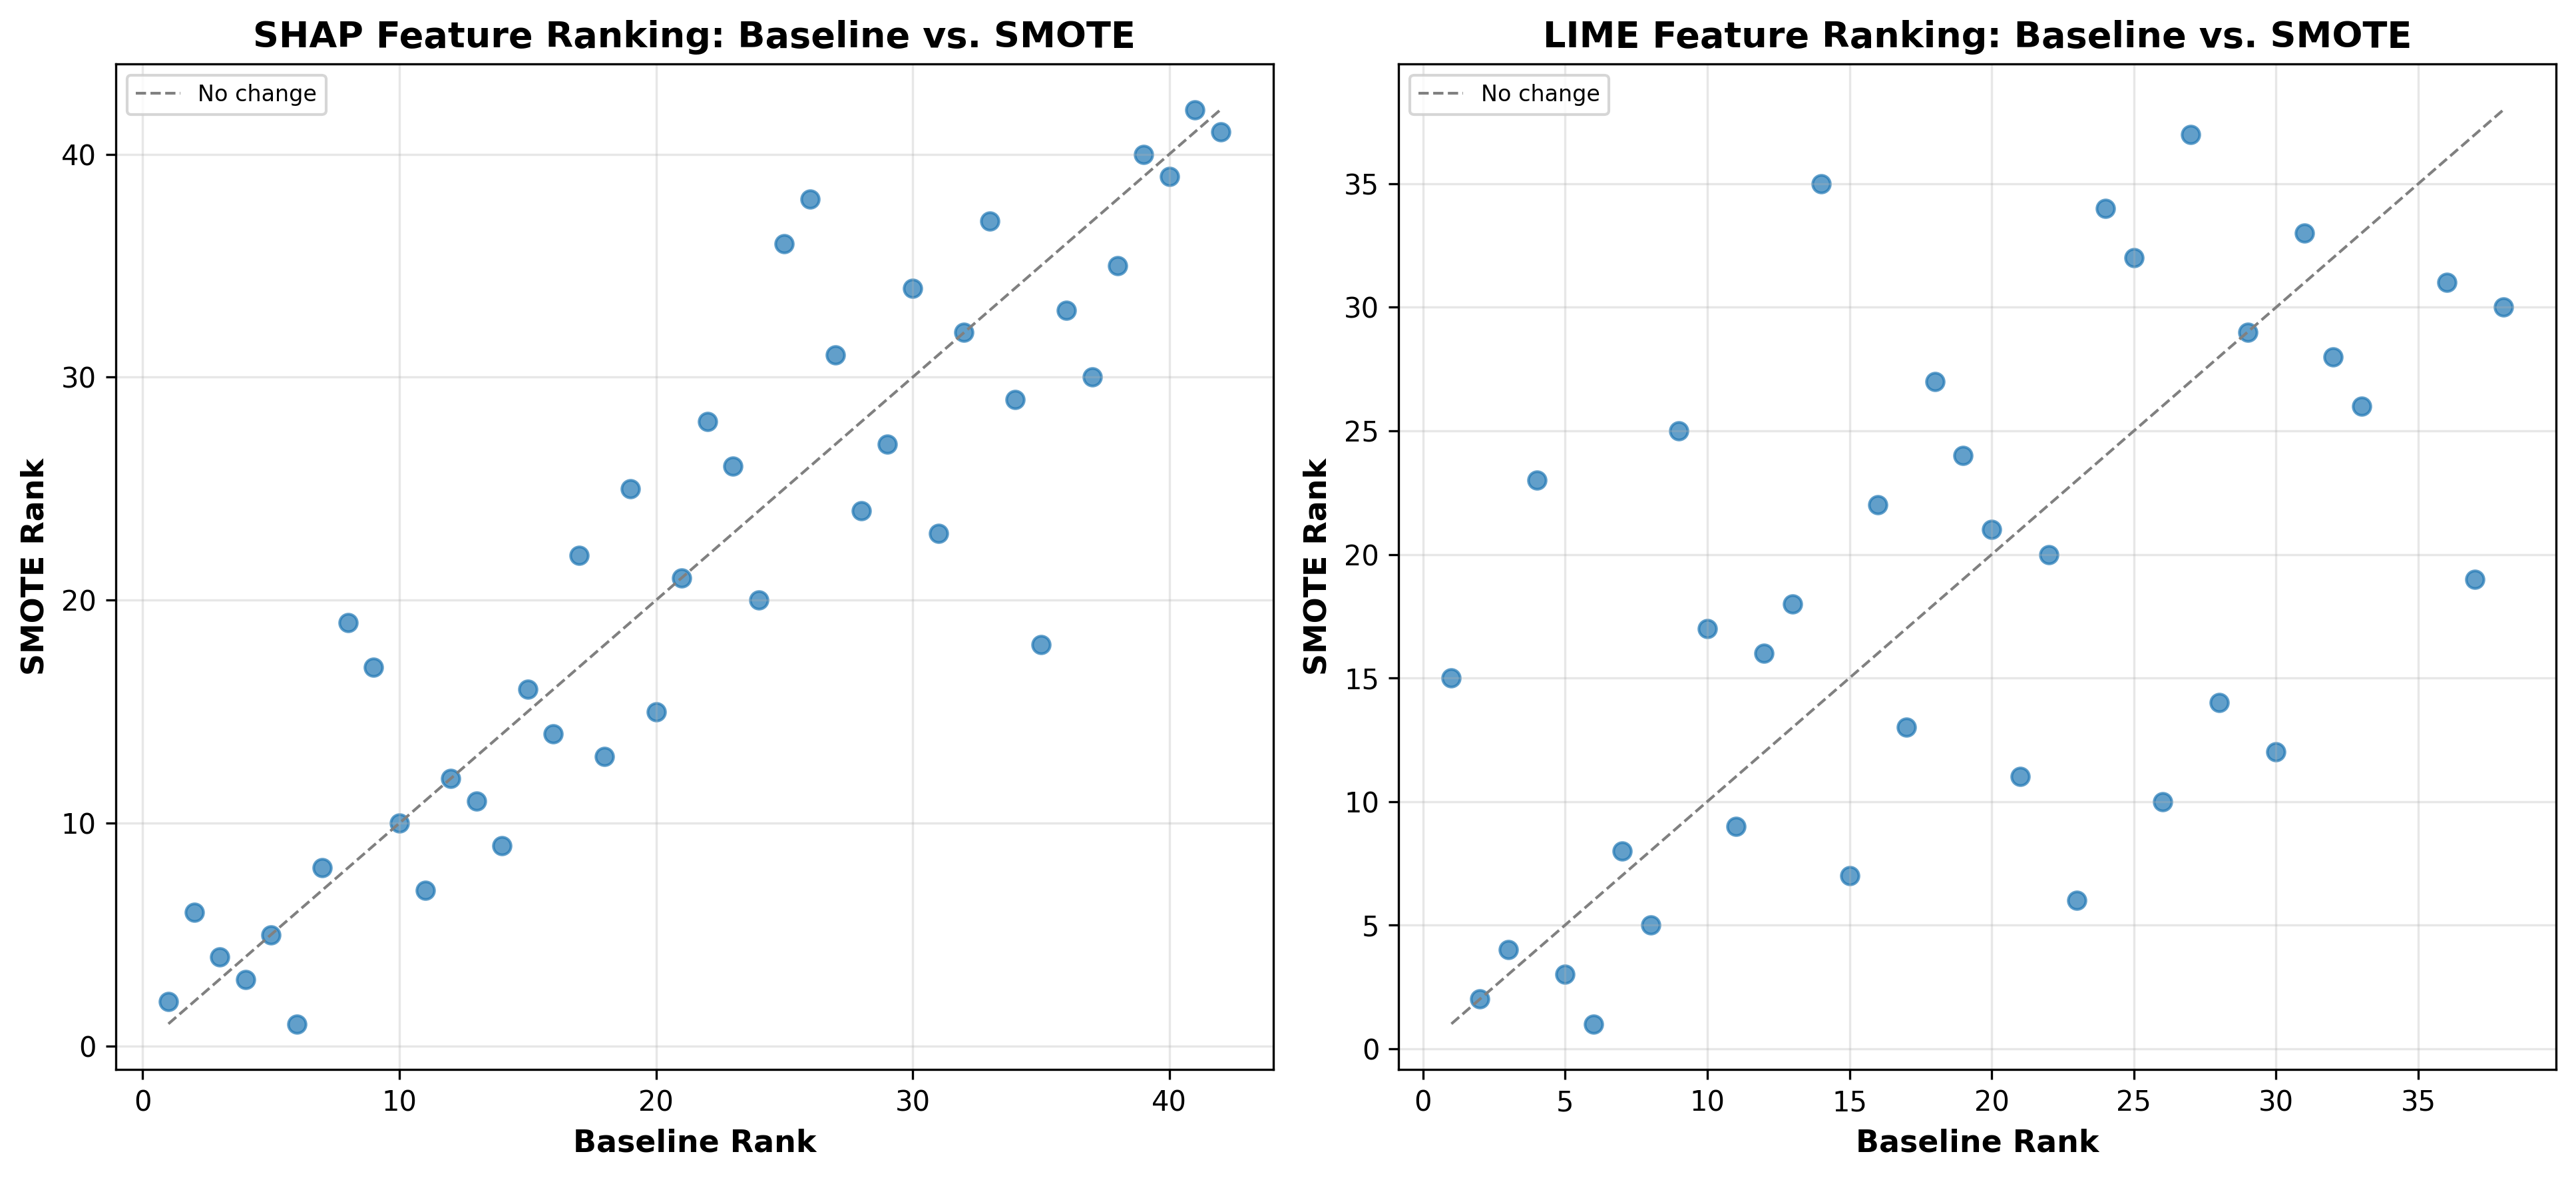
\includegraphics[width=\textwidth]{explanation_ranking_comparison.png}
  \caption{Feature rank comparison: Baseline vs.\ SMOTE for SHAP (top) and LIME
           (bottom). Crossing lines indicate rank-order changes; LIME shows
           greater rank instability.}
  \label{fig:ranking}
\end{figure*}

\begin{figure*}[b]
  \centering
  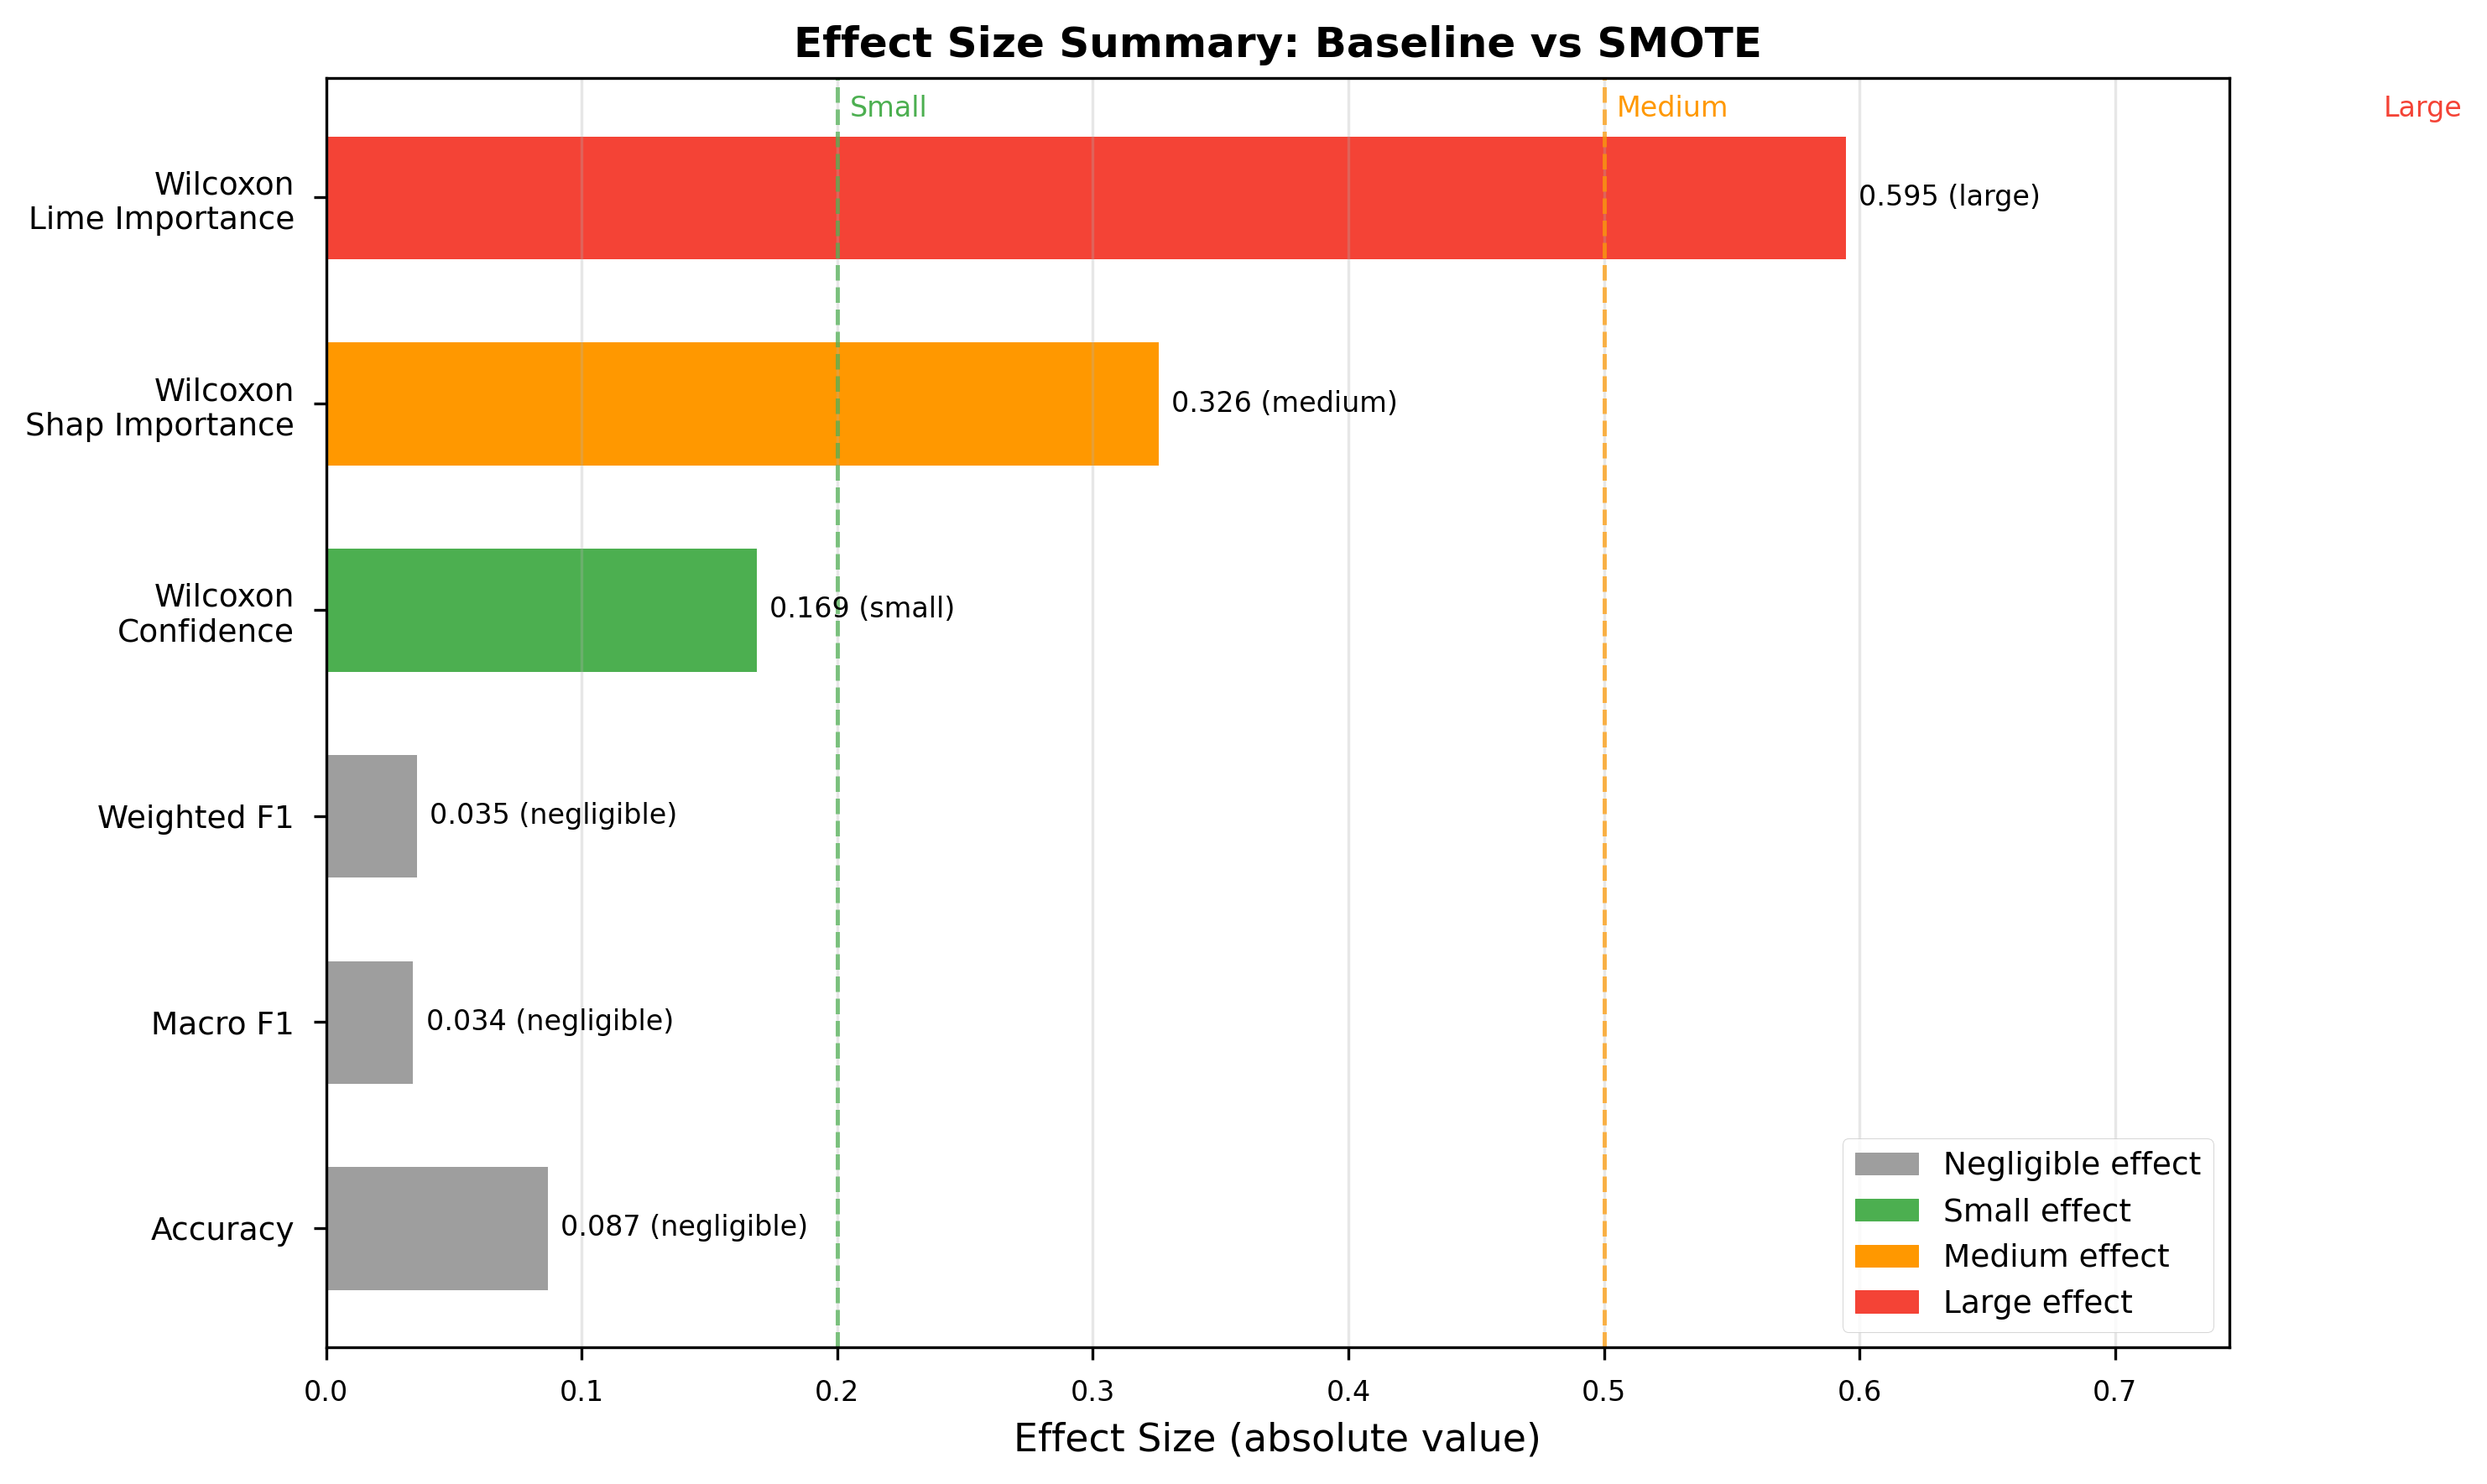
\includegraphics[width=\textwidth]{effect_sizes.png}
  \caption{Effect size summary. \cohensh (predictive metrics, left) and
           rank-biserial~$r$ (Wilcoxon tests on feature importances, right).
           All predictive effects are negligible ($|h|\leq 0.087$); explanatory
           effects range from small to large ($r=0.169$--$0.595$). Note: the two
           metrics operate on different scales and sample sizes; the figure
           illustrates qualitative asymmetry, not a precise proportional ratio.}
  \label{fig:effect}
\end{figure*}

The central finding is an asymmetry between predictive and explanatory sensitivity
to class rebalancing (Fig.~\ref{fig:effect}, Table~\ref{tab:effect}). All
predictive effect sizes are negligible (max $|h|=0.0868$), while explanation
effect sizes range from small (confidence scores, $r=0.1686$) to medium (SHAP,
$r=0.3259$) to large (LIME, $r=0.5947$). LIME's explanatory effect size
($r=0.5947$, large) substantially exceeds the maximum predictive effect size
($|h|=0.0868$, negligible). As these two metrics operate on different scales and
reflect different sample sizes ($n=36$ feature pairs vs.\ $n=82{,}332$ paired
predictions), this comparison indicates a qualitative asymmetry --- explanation
attribution rankings are substantially more sensitive to class rebalancing than
aggregate classification outcomes --- rather than a precise proportional
relationship.

\smallskip
\noindent\textbf{Verdict (RQ3):} Explanatory sensitivity substantially exceeds
predictive sensitivity; LIME attribution rankings exhibited the greatest
sensitivity to class rebalancing of all outputs examined.

% --- TABLE III ---------------------------------------------
\begin{table}[t]
  \caption{Effect Sizes: Baseline vs.\ SMOTE Model ($n_\text{test}=82{,}332$)}
  \label{tab:effect}
  \centering
  \begin{tabular}{llrl}
    \toprule
    \textbf{Comparison} & \textbf{Metric} & \textbf{Value} & \textbf{Magnitude} \\
    \midrule
    Accuracy         & $h$    & $-0.0868$ & Negligible \\
    Macro F1         & $h$    & $+0.0340$ & Negligible \\
    Weighted F1      & $h$    & $-0.0354$ & Negligible \\
    Confidence shift & $r$    & $0.1686$  & Small \\
    SHAP shift       & $r$    & $0.3259$  & Medium \\
    LIME shift       & $r$    & $0.5947$  & Large \\
    \bottomrule
    \multicolumn{4}{l}{\footnotesize $h$ via \eqref{eq:cohenh}; $r$ via
      \eqref{eq:rbs}. Thresholds (Cohen~1988):}\\
    \multicolumn{4}{l}{\footnotesize $|h|$: neg.\ $<0.20$, sm.\ $\geq0.20$,
      med.\ $\geq0.50$, lg.\ $\geq0.80$.}\\
    \multicolumn{4}{l}{\footnotesize $r$: sm.\ $\geq0.10$, med.\ $\geq0.30$,
      lg.\ $\geq0.50$. Cross-row: qualitative.}\\
  \end{tabular}
\end{table}

% ----------------------------------------------------------
\subsection{Hypothesis Test Summary (RQ4)}

All four hypothesis tests rejected $H_0$ after Holm--Bonferroni correction
(Table~\ref{tab:hyp}). The research hypothesis --- that class rebalancing affects
\XAI explanations more than aggregate predictive metrics --- is supported by the
asymmetry between negligible predictive effect sizes and medium-to-large explanation
effect sizes. LIME's greater sensitivity relative to SHAP ($\Delta r=0.269$) is
consistent with the expectation that perturbation-based local explanation methods
are more sensitive to training distribution changes than exact tree-attribution
methods.

% --- TABLE IV ----------------------------------------------
\begin{table}[t]
  \caption{Hypothesis Test Summary (Holm--Bonferroni Corrected,
           $\alpha=0.05$, Four Tests)}
  \label{tab:hyp}
  \centering
  \begin{tabular}{lllrl}
    \toprule
    \textbf{Test} & \textbf{Statistic} &
      \bm{$p$}\textbf{-value} & \textbf{Holm~}$\bm{\alpha}$ &
      \textbf{Reject} \\
    \midrule
    McNemar (Yates)   & $\chi^2=1547.51$ & $<10^{-300}$ & 0.0125 & Yes \\
    Wilcoxon (conf.)  & $W=455{,}648{,}244$& $<10^{-300}$ & 0.0167 & Yes \\
    Wilcoxon (LIME)   & $W=115.0$        & $3.59\times10^{-4}$ & 0.0250 & Yes \\
    Wilcoxon (SHAP)   & $W=283.0$        & $3.47\times10^{-2}$ & 0.0500 & Yes \\
    \bottomrule
    \multicolumn{5}{l}{\footnotesize Ordered by Holm rank. $b=1{,}632$,
      $c=4{,}784$ (McNemar).}\\
    \multicolumn{5}{l}{\footnotesize SHAP power $\approx0.55$ ($n=42$);
      LIME power $\approx0.90$ ($n=36$).}\\
  \end{tabular}
\end{table}

% ==========================================================
\section{Discussion}
\label{sec:discussion}
% ==========================================================

\subsection{Interpretation of Findings}

The central finding --- that \SMOTE changes explanation structure more than
prediction structure --- has an intuitive interpretation. Class rebalancing
redistributes the model's learned decision boundary: minority classes, previously
under-represented, receive proportionally more training signal. Even when aggregate
classification accuracy remains essentially unchanged, the model's internal feature
weighting shifts to accommodate the new distribution. Post-hoc explanation methods
detect this shift directly, because they query the model's local decision surface
rather than summarising outputs with a single metric. This is consistent with LIME
being more sensitive than SHAP: LIME evaluates the model on perturbed local
neighbourhoods, which are directly affected by the shifted decision boundary,
whereas SHAP computes global Shapley-value attributions that partially average out
local perturbations.

\subsection{Practical Implications}

\begin{enumerate}
  \item \textbf{Cybersecurity practitioners:} Accuracy alone is insufficient to
        validate retraining. Explanation outputs may change substantially even if
        accuracy changes are negligible. Practitioners should re-validate \XAI
        outputs after any retraining event.
  \item \textbf{Intrusion detection deployment:} \SMOTE improves minority-class
        detection (Worms F1: $0.233\to0.452$) at a measurable cost: of 82,332
        instances, \SMOTE gained 1,632 (1.98\%) predictions but lost 4,784
        (5.81\%). For rare-attack-priority deployments this trade-off may be
        acceptable; for false-positive-sensitive environments it warrants careful
        consideration.
  \item \textbf{Model transparency:} LIME-based explanations are substantially
        more sensitive to training distribution than SHAP-based explanations.
        Practitioners should be aware that a distribution change can produce a
        large shift ($r=0.595$) in LIME rankings without a corresponding change
        in model accuracy.
  \item \textbf{Trustworthy AI:} \XAI pipelines should include
        explanation-consistency monitoring alongside accuracy monitoring.
  \item \textbf{Operational monitoring:} Retraining-triggered explanation audits
        should be standard practice. Tracking Spearman correlation of feature
        rankings before and after retraining may detect explanation drift that
        accuracy-only monitoring misses.
\end{enumerate}

\subsection{Relationship to Trustworthy AI}

The asymmetry between predictive and explanatory sensitivity has direct implications
for trustworthy-AI frameworks in cybersecurity \cite{charmet2022,rjoub2023}.
Regulatory guidance on AI transparency increasingly requires that explanations be
provided for consequential decisions \cite{euaiact2024}. If those explanations are
unstable under routine model updates such as rebalancing, the explanations
themselves become unreliable, even when performance metrics remain acceptable.
To the best of the authors' knowledge, this study provides the first empirical
evidence of this instability in a standardised \NIDS benchmark setting.

% ==========================================================
\section{Limitations}
\label{sec:limitations}
% ==========================================================

\subsection{Internal Validity}

\begin{itemize}
  \item \textbf{Single rebalancing technique:} Only \SMOTE was evaluated. Other
        techniques (ADASYN, cost-sensitive learning, undersampling, ensemble
        methods) may produce different explanatory outcomes.
  \item \textbf{Single model family:} Random Forest was the only classifier
        evaluated. SHAP TreeExplainer is specific to tree-based models; LIME's
        sensitivity may differ for neural networks or SVMs.
  \item \textbf{Explanation subset size and statistical power:} \XAI explanations
        were computed on 60 instances. Wilcoxon tests used $n=42$ (SHAP) and
        $n=36$ (LIME) paired feature pairs. At $n=42$, power to detect the
        observed SHAP effect ($r=0.326$) is $\approx 0.55$, below the conventional
        0.80 threshold; a non-significant result at this sample size would not
        have been conclusive. At $n=36$, power to detect the LIME effect
        ($r=0.595$) is $\approx 0.90$.
  \item \textbf{LIME surrogate fidelity:} Mean local $R^2$ was 0.290 (Baseline)
        and 0.252 (SMOTE). The ranking shift ($r=0.5947$) is statistically
        robust; however, absolute LIME weights should not be interpreted as exact
        attributions.
\end{itemize}

\subsection{External Validity}

\begin{itemize}
  \item \textbf{Single dataset and temporal scope:} UNSW-NB15 was captured in a
        controlled laboratory environment and released in 2015. Network attack
        techniques, protocol distributions, and adversarial strategies have evolved
        considerably; contemporary enterprise environments carry encrypted TLS~1.3
        traffic, microservice-to-microservice communication, and cloud API patterns
        not represented in this dataset. Findings are valid within the scope of
        UNSW-NB15 as a standardised benchmark; transferability to modern
        environments warrants validation on more recent captures (e.g.,
        CICIDS-2017, CSE-CIC-IDS-2018).
  \item \textbf{Synthetic minority samples:} \SMOTE generated 384,659 synthetic
        samples. These instances may not faithfully represent real attack traffic
        in production networks.
  \item \textbf{Static dataset:} Concept drift in live network traffic may
        invalidate both predictive performance and explanation patterns.
\end{itemize}

\subsection{Construct Validity}

\begin{itemize}
  \item \textbf{Operationalisation of explanation quality:} Quality is
        operationalised as feature rank stability (Spearman $\rho$, top-$k$
        overlap) and importance magnitude shift (Wilcoxon). Human interpretability
        and ground-truth fidelity are not evaluated.
  \item \textbf{SHAP vs.\ LIME comparability:} SHAP values are additive
        attributions; LIME weights are local linear approximation coefficients.
        Their rank-biserial $r$ values are not directly commensurate.
  \item \textbf{Worms class sample size:} The Worms test class contains only
        44~instances. F1 comparisons at this scale are reported as indicative
        results.
\end{itemize}

% ==========================================================
\section{Future Work}
\label{sec:future}
% ==========================================================

Future work should address: (i) alternative rebalancing techniques (ADASYN,
class-weighted loss) to generalise the explanation-shift finding; (ii)
gradient-based SHAP and Integrated Gradients for neural network \NIDS models;
(iii) multi-dataset validation (CICIDS-2017, NSL-KDD) for generalisability;
(iv) human-centred evaluation of whether observed rank shifts affect analyst
decision-making; and (v) formal explanation-consistency metrics for \NIDS
model certification.

% ==========================================================
\section{Conclusion}
\label{sec:conclusion}
% ==========================================================

This paper presented a controlled empirical investigation into the impact of
\SMOTE-based class rebalancing on the predictive performance and \XAI explanation
quality of a Random Forest--based \NIDS trained on the UNSW-NB15 benchmark.
Statistical analysis of 82,332 paired test-set predictions demonstrated that
\SMOTE produces statistically significant but practically negligible changes to
aggregate predictive metrics (max $|h|=0.087$), while producing medium-to-large
changes to SHAP and LIME feature attribution rankings (rank-biserial $r$ up to
0.595 for LIME).

The primary finding --- that LIME explanation sensitivity to class rebalancing
substantially and disproportionately exceeds predictive sensitivity across
complementary effect-size measures --- demonstrates that accuracy-only validation
is insufficient for \XAI-augmented \NIDS pipelines. This finding holds even with
the caveat that LIME local surrogate fidelity ($R^2\approx0.25$--$0.29$) is
moderate: the statistical evidence for a large explanatory shift is robust
regardless of absolute attribution magnitudes.

The secondary finding --- that LIME is more sensitive than SHAP to training
distribution changes --- has methodological implications for \XAI tool selection:
perturbation-based local explanation methods should be independently validated when
training data composition changes, and their surrogate fidelity should be reported
alongside attribution rankings.

Future work should validate these findings across additional datasets, model
families, and rebalancing strategies to establish the generalisability of
explanation-consistency monitoring as a practical component of trustworthy \NIDS
development.

% ==========================================================
%  REFERENCES  (IEEE appearance order)
% ==========================================================
\begin{thebibliography}{23}

\bibitem{alshamy2021}
R.~Alshamy, M.~Ghurab, S.~Othman, and F.~Alshami,
``Intrusion detection model for imbalanced dataset using SMOTE and random
forest algorithm,''
in \emph{Advances in Cyber Security (ACeS~2021)},
ser. Commun. Comput. Inf. Sci. (CCIS), vol.~1487.
Singapore: Springer, 2021, pp.~311--323.
doi:~10.1007/978-981-16-8059-5\_22.

\bibitem{wu2022}
T.~Wu, H.~Fan, H.~Zhu, C.~You, H.~Zhou, and X.~Huang,
``Intrusion detection system combined enhanced random forest with SMOTE
algorithm,''
\emph{EURASIP J. Adv. Signal Process.}, vol.~2022, Art. no.~39, 2022.
doi:~10.1186/s13634-022-00871-6.

\bibitem{more2024}
S.~More, M.~Idrissi, H.~Mahmoud, and A.~T.~Asyhari,
``Enhanced intrusion detection systems performance with UNSW-NB15 data
analysis,''
\emph{Algorithms}, vol.~17, no.~2, Art. no.~64, Feb. 2024.
doi:~10.3390/a17020064.

\bibitem{moustafa2015}
N.~Moustafa and J.~Slay,
``UNSW-NB15: A comprehensive data set for network intrusion detection
systems,''
in \emph{Proc. IEEE Military Commun. Inf. Syst. Conf. (MilCIS)},
Canberra, Australia, Nov. 2015, pp.~1--6.
doi:~10.1109/MilCIS.2015.7348942.

\bibitem{shanmugam2025}
V.~Shanmugam, R.~Razavi-Far, and E.~Hallaji,
``Addressing class imbalance in intrusion detection: A comprehensive
evaluation of machine learning approaches,''
\emph{Electronics}, vol.~14, no.~1, Art. no.~69, Jan. 2025.
doi:~10.3390/electronics14010069.

\bibitem{chawla2002}
N.~V.~Chawla, K.~W.~Bowyer, L.~O.~Hall, and W.~P.~Kegelmeyer,
``SMOTE: Synthetic minority over-sampling technique,''
\emph{J. Artif. Intell. Res.}, vol.~16, pp.~321--357, Jun. 2002.
doi:~10.1613/jair.953.

\bibitem{sayegh2024}
H.~R.~Sayegh, W.~Dong, and A.~M.~Al-madani,
``Enhanced intrusion detection with LSTM-based model, feature selection,
and SMOTE for imbalanced data,''
\emph{Appl. Sci.}, vol.~14, no.~2, Art. no.~479, Jan. 2024.
doi:~10.3390/app14020479.

\bibitem{charmet2022}
F.~Charmet, H.~C.~Tanuwidjaja, S.~Ayoubi, P.~F.~Gimenez, Y.~Han,
H.~Jmila \emph{et~al.},
``Explainable artificial intelligence for cybersecurity: A literature
survey,''
\emph{Ann. Telecommun.}, vol.~77, no.~11--12, pp.~789--812, 2022.
doi:~10.1007/s12243-022-00926-7.

\bibitem{rjoub2023}
G.~Rjoub, J.~Bentahar, O.~Abdel~Wahab, R.~Mizouni, A.~Song,
R.~Cohen \emph{et~al.},
``A survey on explainable artificial intelligence for cybersecurity,''
\emph{IEEE Trans. Netw. Serv. Manag.}, vol.~20, no.~4,
pp.~5115--5140, Dec. 2023.
doi:~10.1109/TNSM.2023.3282740.

\bibitem{lundberg2017}
S.~M.~Lundberg and S.-I.~Lee,
``A unified approach to interpreting model predictions,''
in \emph{Adv. Neural Inf. Process. Syst. (NeurIPS)}, vol.~30,
Long Beach, CA, USA, Dec. 2017, pp.~4766--4777. [Online]. Available:
\url{https://proceedings.neurips.cc/paper_files/paper/2017/hash/%
8a20a8621978632d76c43dfd28b67767-Abstract.html}

\bibitem{lundberg2020}
S.~M.~Lundberg, G.~Erion, H.~Chen, A.~DeGrave, J.~M.~Prutkin,
B.~Nair \emph{et~al.},
``From local explanations to global understanding with explainable AI
for trees,''
\emph{Nat. Mach. Intell.}, vol.~2, no.~1, pp.~56--67, Jan. 2020.
doi:~10.1038/s42256-019-0138-9.

\bibitem{ribeiro2016}
M.~T.~Ribeiro, S.~Singh, and C.~Guestrin,
```Why should I trust you?': Explaining the predictions of any
classifier,''
in \emph{Proc. 22nd ACM SIGKDD Int. Conf. Knowl. Discovery Data Mining
(KDD)}, San Francisco, CA, USA, Aug. 2016, pp.~1135--1144.
doi:~10.1145/2939672.2939778.

\bibitem{gaspar2024}
D.~Gaspar, P.~Silva, and C.~Silva,
``Explainable AI for intrusion detection systems: LIME and SHAP
applicability on multi-layer perceptron,''
\emph{IEEE Access}, vol.~12, pp.~30164--30175, 2024.
doi:~10.1109/ACCESS.2024.3368377.

\bibitem{hermosilla2025a}
P.~Hermosilla, S.~Berr\'ios, and H.~Allende-Cid,
``Explainable AI for forensic analysis: A comparative study of SHAP and
LIME in intrusion detection models,''
\emph{Appl. Sci.}, vol.~15, no.~13, Art. no.~7329, Jul. 2025.
doi:~10.3390/app15137329.

\bibitem{hermosilla2025b}
P.~Hermosilla, M.~D\'iaz, S.~Berr\'ios, and H.~Allende-Cid,
``Use of explainable artificial intelligence for analyzing and explaining
intrusion detection systems,''
\emph{Computers}, vol.~14, no.~5, Art. no.~160, May 2025.
doi:~10.3390/computers14050160.

\bibitem{visani2022}
G.~Visani, E.~Bagli, F.~Chesani, A.~Poluzzi, and D.~Capuzzo,
``Statistical stability indices for LIME: Obtaining reliable explanations
for machine learning models,''
\emph{J. Oper. Res. Soc.}, vol.~73, no.~1, pp.~91--101, 2022.
doi:~10.1080/01605682.2020.1865846.

\bibitem{patil2020}
A.~Patil, A.~Framewala, and F.~Kazi,
``Explainability of SMOTE based oversampling for imbalanced dataset
problems,''
in \emph{Proc. IEEE Int. Conf. Inf. Commun. Technol. (ICICT)},
San Jose, CA, USA, Feb. 2020, pp.~41--45.
doi:~10.1109/ICICT50521.2020.9092325.

\bibitem{alarab2022}
I.~Alarab and S.~Prakoonwit,
``Effect of data resampling on feature importance in imbalanced blockchain
data: Comparison studies of resampling techniques,''
\emph{Data Sci. Manag.}, vol.~5, no.~2, pp.~66--76, Jun. 2022.
doi:~10.1016/j.dsm.2022.04.003.

\bibitem{breiman2001}
L.~Breiman,
``Random forests,''
\emph{Mach. Learn.}, vol.~45, no.~1, pp.~5--32, Oct. 2001.
doi:~10.1023/A:1010933404324.

\bibitem{virtanen2020}
P.~Virtanen, R.~Gommers, T.~E.~Oliphant, M.~Haberland, T.~Reddy,
D.~Cournapeau \emph{et~al.},
``SciPy~1.0: Fundamental algorithms for scientific computing in Python,''
\emph{Nat. Methods}, vol.~17, pp.~261--272, Feb. 2020.
doi:~10.1038/s41592-020-0772-5.

\bibitem{pedregosa2011}
F.~Pedregosa, G.~Varoquaux, A.~Gramfort, V.~Michel, B.~Thirion,
O.~Grisel \emph{et~al.},
``Scikit-learn: Machine learning in Python,''
\emph{J. Mach. Learn. Res.}, vol.~12, pp.~2825--2830, Nov. 2011.
[Online]. Available: \url{http://jmlr.org/papers/v12/pedregosa11a.html}

\bibitem{lemaitre2017}
G.~Lema\^{i}tre, F.~Nogueira, and C.~K.~Aridas,
``Imbalanced-learn: A Python toolbox to tackle the curse of imbalanced
datasets in machine learning,''
\emph{J. Mach. Learn. Res.}, vol.~18, no.~17, pp.~1--5, 2017.
[Online]. Available: \url{http://jmlr.org/papers/v18/16-365.html}

\bibitem{euaiact2024}
European Parliament and Council of the European Union,
``Regulation (EU) 2024/1689 laying down harmonised rules on artificial
intelligence (Artificial Intelligence Act),''
\emph{Off. J. Eur. Union}, Jul. 2024. [Online]. Available:
\url{https://eur-lex.europa.eu/legal-content/EN/TXT/?uri=CELEX:32024R1689}

\end{thebibliography}

% ==========================================================
\end{document}
% ==========================================================
